\documentclass{article}
%\usepackage[a4paper,margin=1in,landscape]{geometry}
\usepackage{blindtext}
\usepackage{tikz}
\usetikzlibrary{calc}
\usepackage{wrapfig}
\usepackage{enumitem}
\usepackage[paperheight=8.25in,paperwidth=8.25in,margin=1in]{geometry}
\usepackage{fancyhdr}
\usepackage{graphicx}
\usepackage{lipsum}
\usepackage{gensymb}


\title{Cookbook}
\author{Arthur}
\date{ }



\pagestyle{fancy}
\fancyhead{}
\fancyfoot{}
% Set the right side of the footer to be the page number
\fancyfoot[L]{\thepage}
\renewcommand{\headrulewidth}{0pt}




\begin{document}

\maketitle


\newpage
\tableofcontents
 
\newlength{\imagewidth}  % the name can be chosen, e.g. picwidth...

\newpage
\section*{\fontsize{25}{15}\selectfont Introduction}
\addcontentsline{toc}{section}{Introduction}

Cook book introduciton and pamble

Lorem ipsum dolor sit amet, consectetur adipiscing elit. Suspendisse vitae justo tempor, tincidunt diam et, mattis nulla. Vivamus a odio eros. Curabitur sed nisi felis. Aliquam a dolor ac nunc dictum cursus. Suspendisse potenti. Vivamus id eleifend dolor, cursus fringilla nulla. Etiam non nisl arcu. Ut ut tortor ut erat euismod sodales.

Vivamus maximus elit mi, egestas egestas eros accumsan eget. Aliquam eget lacus id massa pellentesque dignissim vel sed arcu. Nam eget est lectus. Vestibulum ante ipsum primis in faucibus orci luctus et ultrices posuere cubilia Curae; Maecenas congue finibus aliquam. Nullam ullamcorper ipsum eget tincidunt vestibulum. Cum sociis natoque penatibus et magnis dis parturient montes, nascetur ridiculus mus. Donec vestibulum quis neque sed rhoncus. Pellentesque habitant morbi tristique senectus et netus et malesuada fames ac turpis egestas. Quisque id blandit nulla. Vestibulum quis nunc at nulla tristique commodo accumsan quis ex. Quisque non odio ullamcorper, suscipit turpis eu, finibus nulla. Quisque condimentum mi elementum mi tempus tincidunt.



%%%%%%%%%%%%%%%%%%%%%%%%%%%%%%%%%%%%%%%%%%%%%%%%%%%%%%%%%%%%%%%%%%%%%%%%%%%%%%%%%%%%%%%%%%%%%%%%%%%%%%%%%%%%%%%%%%%%%%%%%%%%%%%%%%%
% recipe format

%title picture add file name twice

\settowidth{\imagewidth}{\includegraphics{/home/rachel/Documents/Cookbook/Pictures/20151107_191308.jpg}}
\newgeometry{left=0cm,bottom=0cm,top=0cm,right=0cm}
\newpage
\begin{figure}[]
\includegraphics[trim = 0 0 0.25\imagewidth{} 0, clip=true, width=\textwidth]{/home/rachel/Documents/Cookbook/Pictures/20151107_191308.jpg}
\end{figure}
\restoregeometry
\clearpage
\newpage
\newgeometry{right=0cm}



% recipe title
\section*{\fontsize{25}{15}\selectfont Recipe format}
\addcontentsline{toc}{section}{Recipe format}



% side figures
\begin{wrapfigure}{r}{0.5\textwidth}
\
  \begin{center}
 	\hfill\begin{minipage}{.5\textwidth}\centering
 	\vspace*{-5.5cm}
		\includegraphics[width=0.8\textwidth]{/home/rachel/Documents/Cookbook/Pictures/20151107_164938.jpg}
		\\[5mm]
		\includegraphics[width=0.8\textwidth]{/home/rachel/Documents/Cookbook/Pictures/20151107_191245.jpg}
		\\[5mm]
		\includegraphics[angle=-90,origin=c, width=0.8\textwidth]{/home/rachel/Documents/Cookbook/Pictures/20151107_185051.jpg}
	\end{minipage}  
	\end{center}

\end{wrapfigure}



% actual recipe
\vspace{10mm}

Lorem ipsum dolor sit amet, consectetur adipiscing elit. In tincidunt enim vel tortor fringilla, non vehicula nisl laoreet. Fusce finibus, sem eget faucibus rutrum, diam libero aliquam mauris, vel vulputate neque mi at sapien. Praesent ultricies felis a augue iaculis, sit amet dignissim velit mollis. In hac habitasse platea dictumst. Suspendisse auctor ultrices ligula ut ullamcorper.
 
\vspace{5mm}
{\fontfamily{lmss}\selectfont 
    \begin{itemize}[noitemsep]
    
      \item[] Lorem ipsum
      \item[] dolor sit
      \item[] amet
      
    \end{itemize}
    }
\vspace{5mm}
    
Nulla scelerisque efficitur arcu sed vestibulum. Donec imperdiet ipsum et placerat cursus. Quisque in mauris eu nunc malesuada bibendum. Aliquam egestas pretium dolor nec dapibus. Nulla interdum ipsum at urna ullamcorper varius. Nunc volutpat lorem sed magna vehicula lobortis. Aliquam sed scelerisque tellus. Quisque vel euismod purus, ac rhoncus nunc.

Maecenas et justo pretium, pulvinar nisl eu, facilisis urna. Etiam fermentum eros non erat porttitor pretium. Morbi efficitur, libero faucibus hendrerit accumsan, ligula tellus pulvinar erat, ac mattis odio turpis eu ex. Morbi ut justo odio. Mauris malesuada et arcu in viverra. Duis sit amet blandit quam, ac dignissim arcu. Etiam finibus pharetra felis et porttitor. Quisque felis erat, posuere nec diam quis, bibendum varius quam.

\restoregeometry




%%%%%%%%%%%%%%%%%%%%%%%%%%%%%%%%%%%%%%%%%%%%%%%%%%%%%%%%%%%%%%%%%%%%%%%%%%%%%%%%%%%%%%%%%%%%%%%%%%%%%%%%%%%%%%%%%%%%%%%%%%%%%%%%%%%
% Pasta Dough

%title picture add file name twice

\settowidth{\imagewidth}{\includegraphics{/home/rachel/Documents/Cookbook/Pictures/20161121_192251.jpg}}
\newgeometry{left=0cm,bottom=0cm,top=0cm,right=0cm}
\newpage
\begin{figure}[]
\includegraphics[trim = 0.25\imagewidth{} 0 0.25\imagewidth{} 350, clip=true, width=\textwidth]{/home/rachel/Documents/Cookbook/Pictures/20161121_192251.jpg}
\end{figure}
\restoregeometry
\clearpage
\newpage
\newgeometry{right=0cm}



% recipe title
\section*{\fontsize{25}{15}\selectfont Fresh Egg Pasta}
\addcontentsline{toc}{section}{Fresh Egg Pasta}

% side figures
\begin{wrapfigure}{r}{0.5\textwidth}
\
  \begin{center}
 	\hfill\begin{minipage}{.5\textwidth}\centering
 	\vspace*{-4.3cm}
		\includegraphics[trim = 800 0 200 0, clip=true, width=0.8\textwidth]{/home/rachel/Documents/Cookbook/Pictures/20161119_161146.jpg}
		\\[5mm]
		\includegraphics[trim = 400 0 800 0, clip=true, width=0.8\textwidth]{/home/rachel/Documents/Cookbook/Pictures/20161119_164202.jpg}
		\\[5mm]
		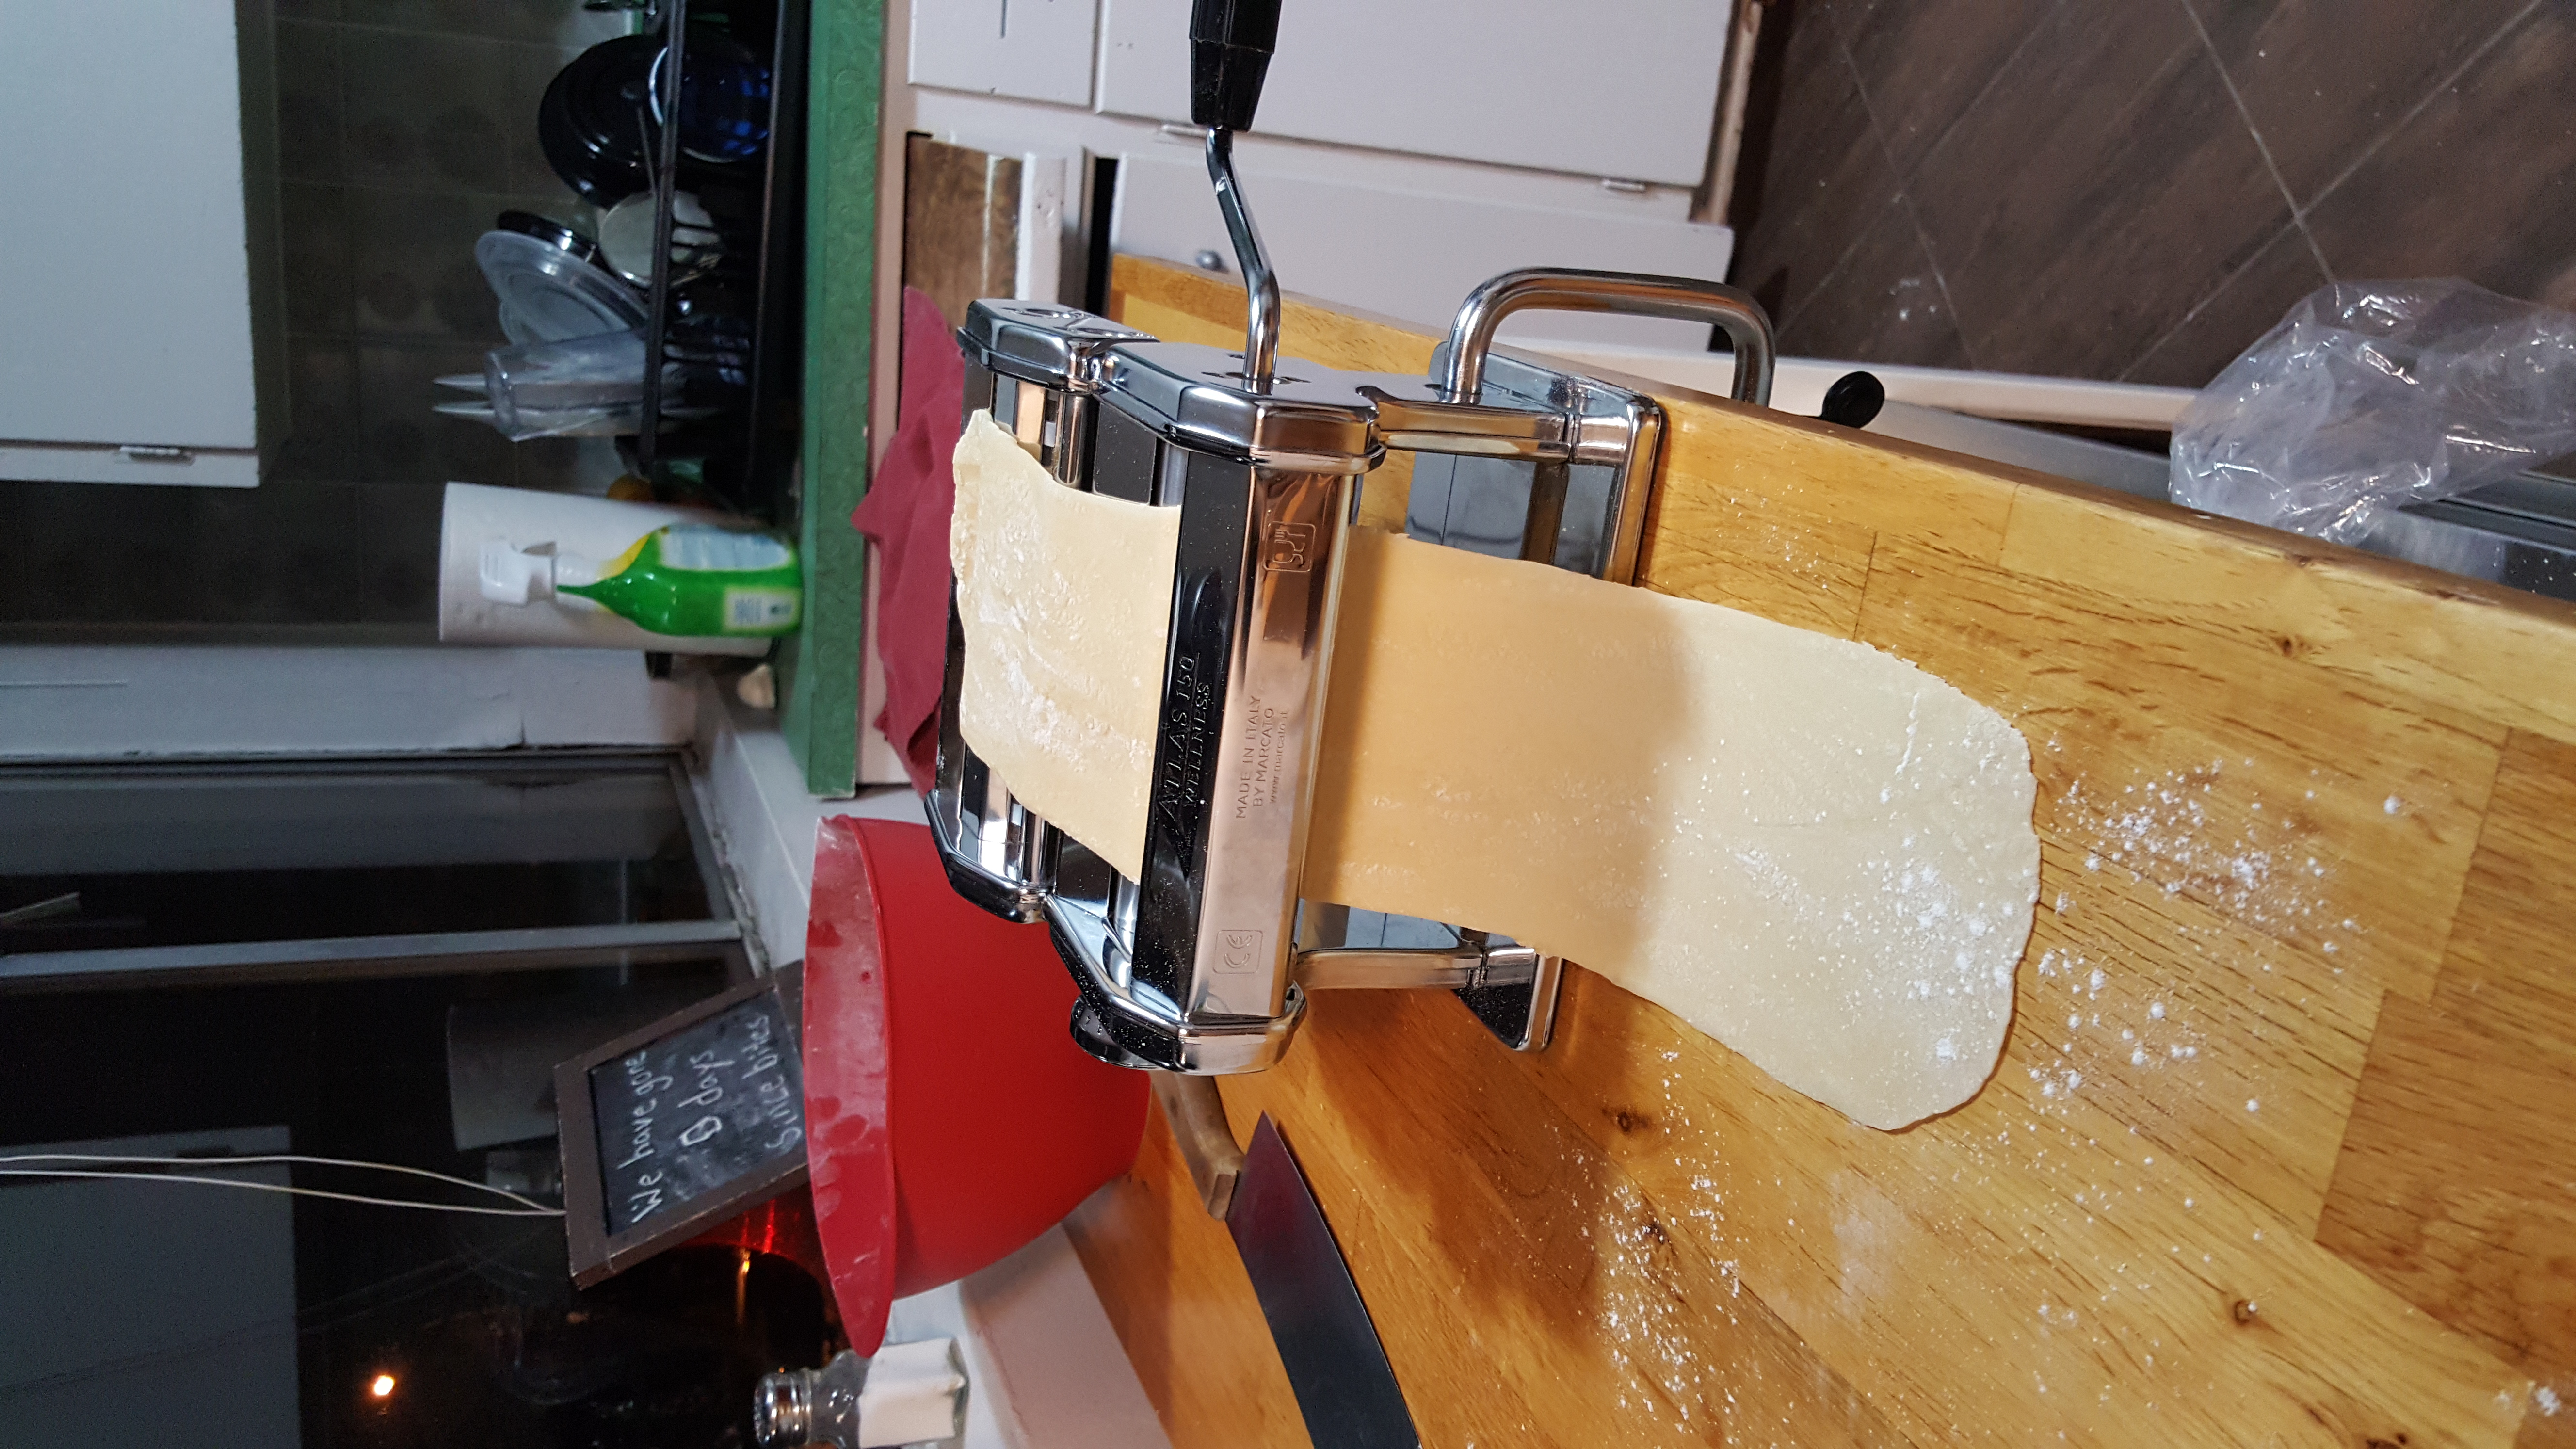
\includegraphics[trim = 800 0 300 0, clip=true, angle=-90,origin=c,width=0.8\textwidth]{/home/rachel/Documents/Cookbook/Pictures/20161121_190803.jpg}
	\end{minipage}  
	\end{center}

\end{wrapfigure}



% actual recipe
\vspace{5mm}

Delicious fresh pasta is a lot more work than dried pasta but so work it. This recipe makes enough for about 4 to 6 servings.

 
\vspace{5mm}
{\fontfamily{lmss}\selectfont 
    \begin{itemize}[noitemsep]
    
      \item[] 2 cups flour, plus extra for rolling the pasta
      \item[] 1/2 teaspoon salt
      \item[] 3 large eggs
      
    \end{itemize}
    }
\vspace{5mm}
    
Combine the flour and salt. Create a deep well in the middle of the flour and crack the eggs into this well. Whisk the eggs with the fork to combine.As you whisk the eggs, begin gradually pulling in flour from the bottom and sides of the well. Don't rush this step. Knead the pasta dough.  Incorporate more flour as needed to prevent the dough from sticking to you or the counter. Slice into the dough with a paring knife; if you see lots of air bubbles, keep kneading. The dough is kneaded when it forms a smooth elastic ball and has very few air bubbles when cut. Approximately ten minutes. Once done place ball of dough inside a floured bowl and cover with a dinner plate or plastic wrap. Rest for at least 30 minutes. 

\textit{Note: At this point, the pasta dough can be refrigerated for up to 24 hours. Let it come back to room temperature before rolling.} 

Sprinkle a baking sheet generously with flour. Divide the dough into four equal portions. Dust the portions with flour and cover with a clean dishtowel.Then make that shit into noodle shapes.

\restoregeometry








%%%%%%%%%%%%%%%%%%%%%%%%%%%%%%%%%%%%%%%%%%%%%%%%%%%%%%%%%%%%%%%%%%%%%%%%%%%%%%%%%%%%%%%%%%%%%%%%%%%%%%%%%%%%%%%%%%%%%%%%%%%%%%%%%%%
% Pasta Sauce

%title picture add file name twice

\settowidth{\imagewidth}{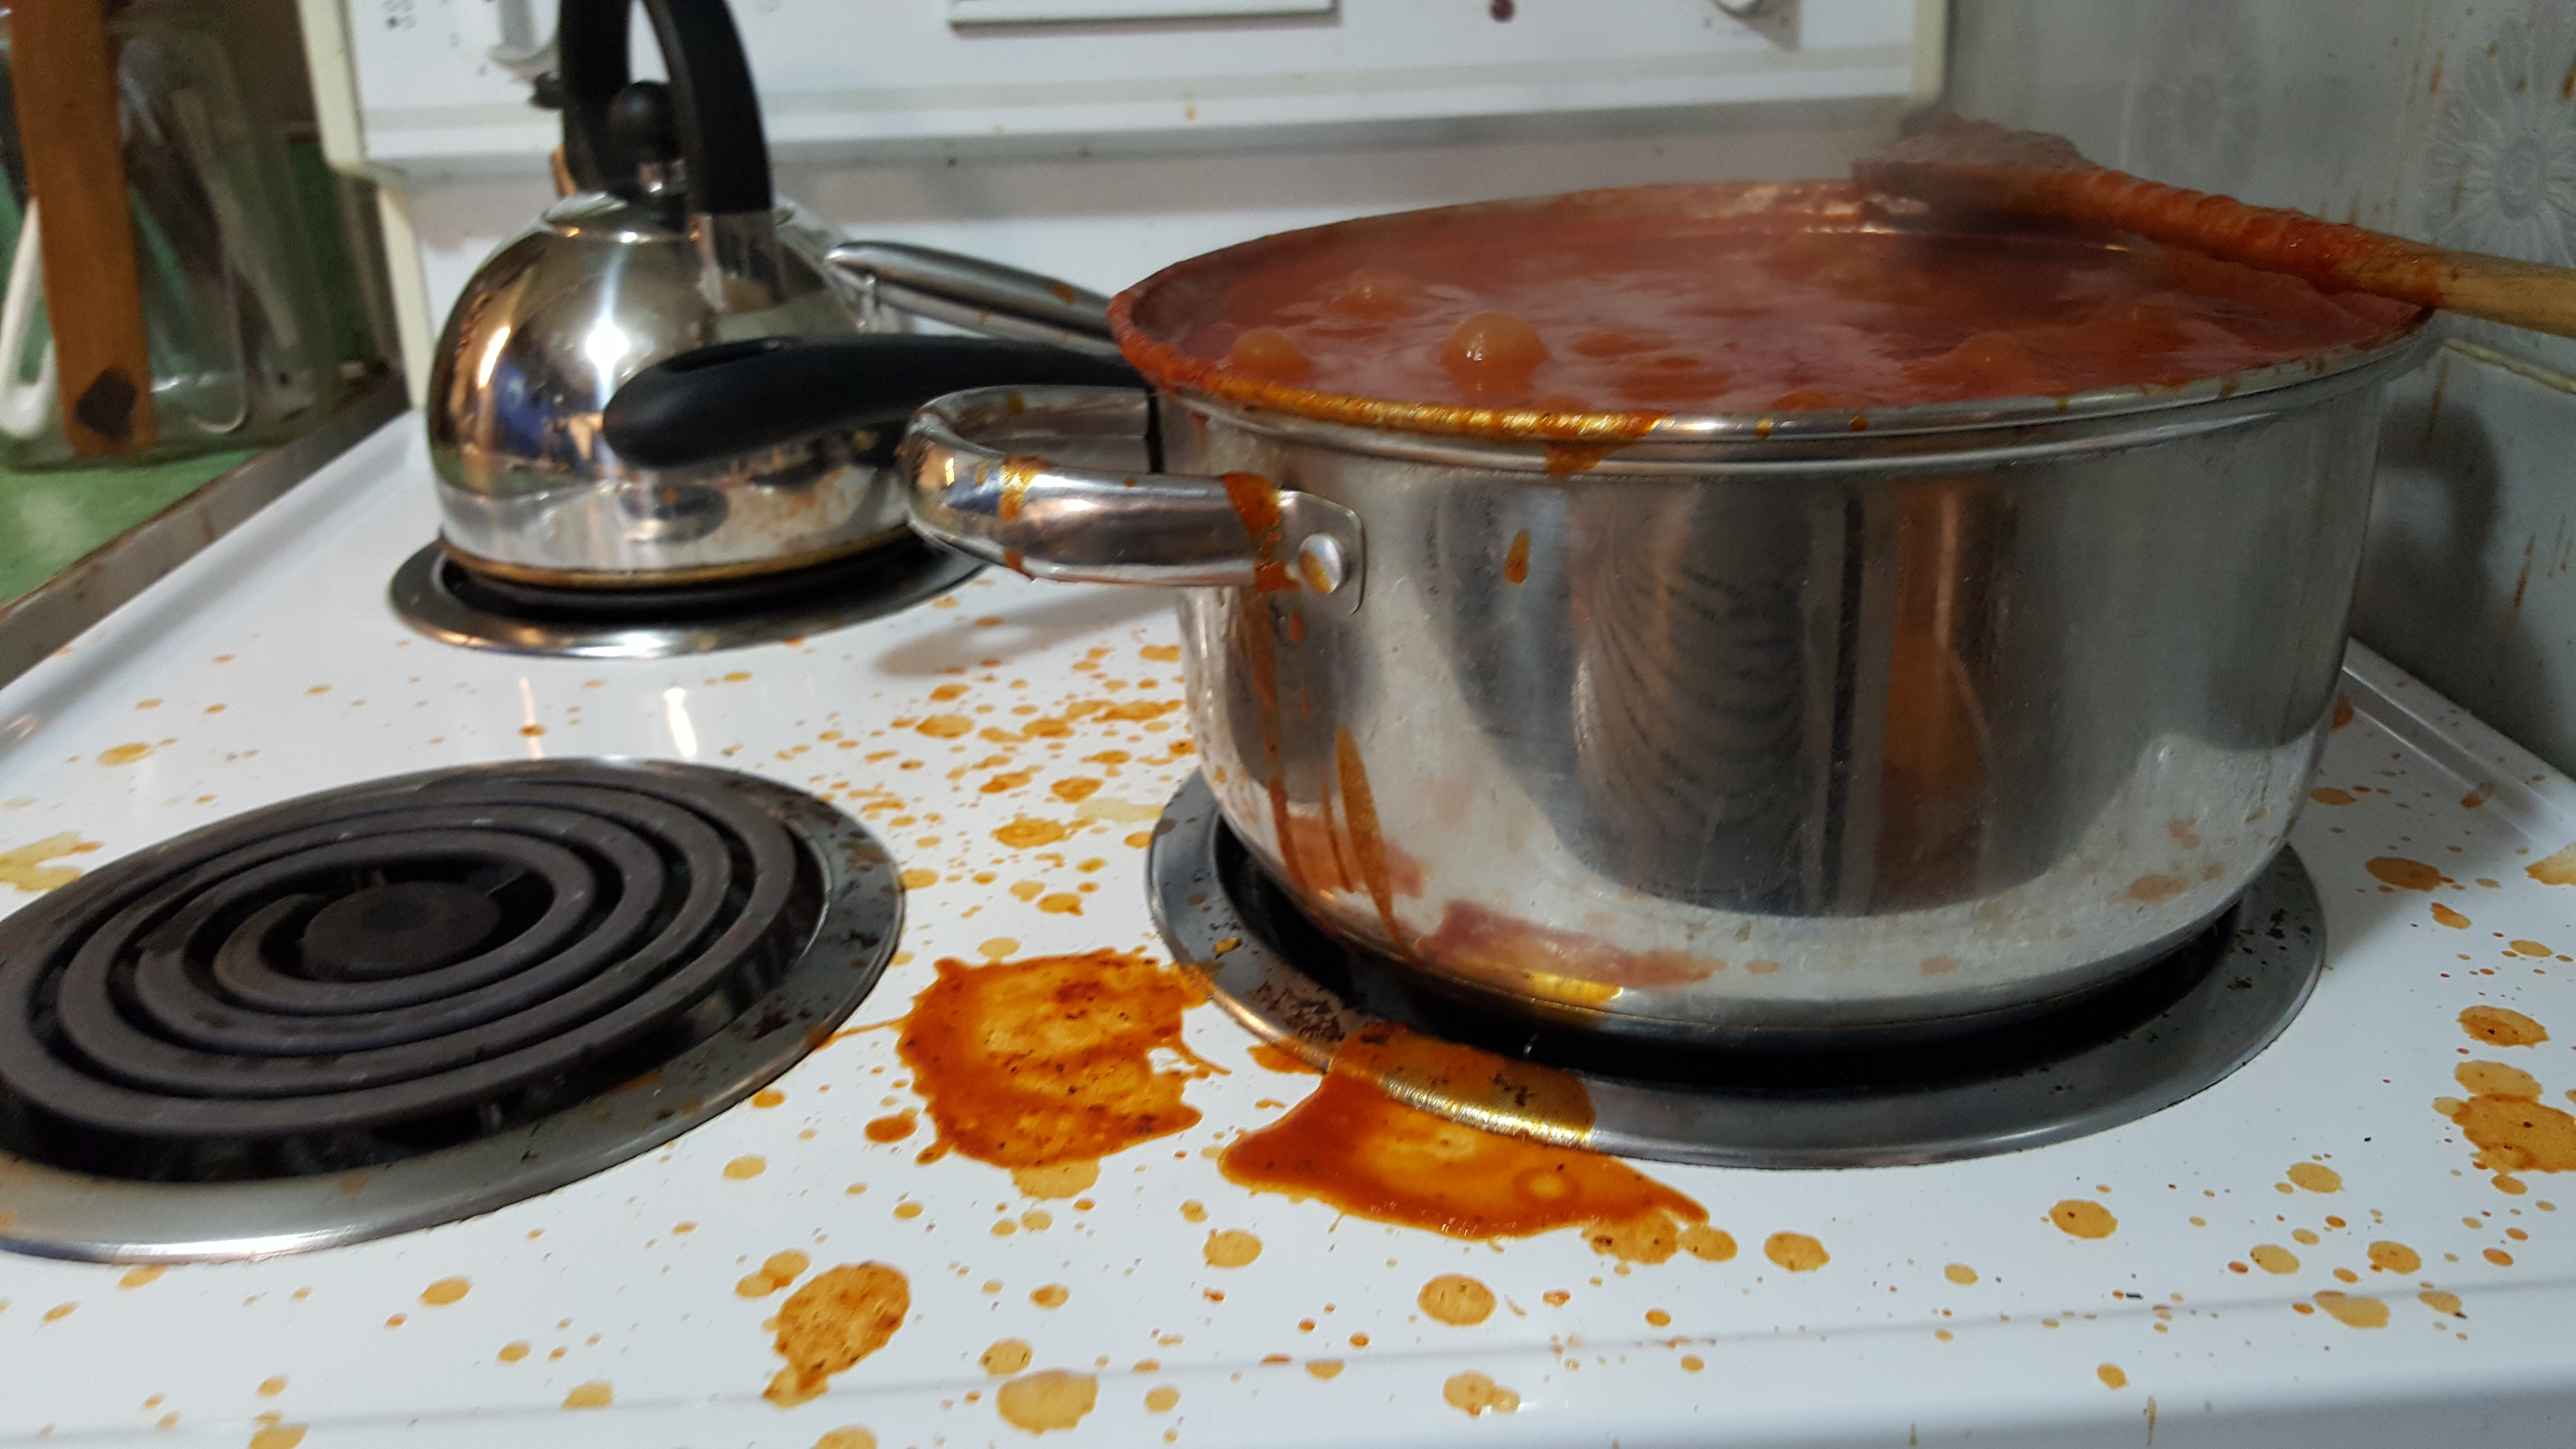
\includegraphics{/home/rachel/Documents/Cookbook/Pictures/20161119_164214.jpg}}
\newgeometry{left=0cm,bottom=0cm,top=0cm,right=0cm}
\newpage
\begin{figure}[]
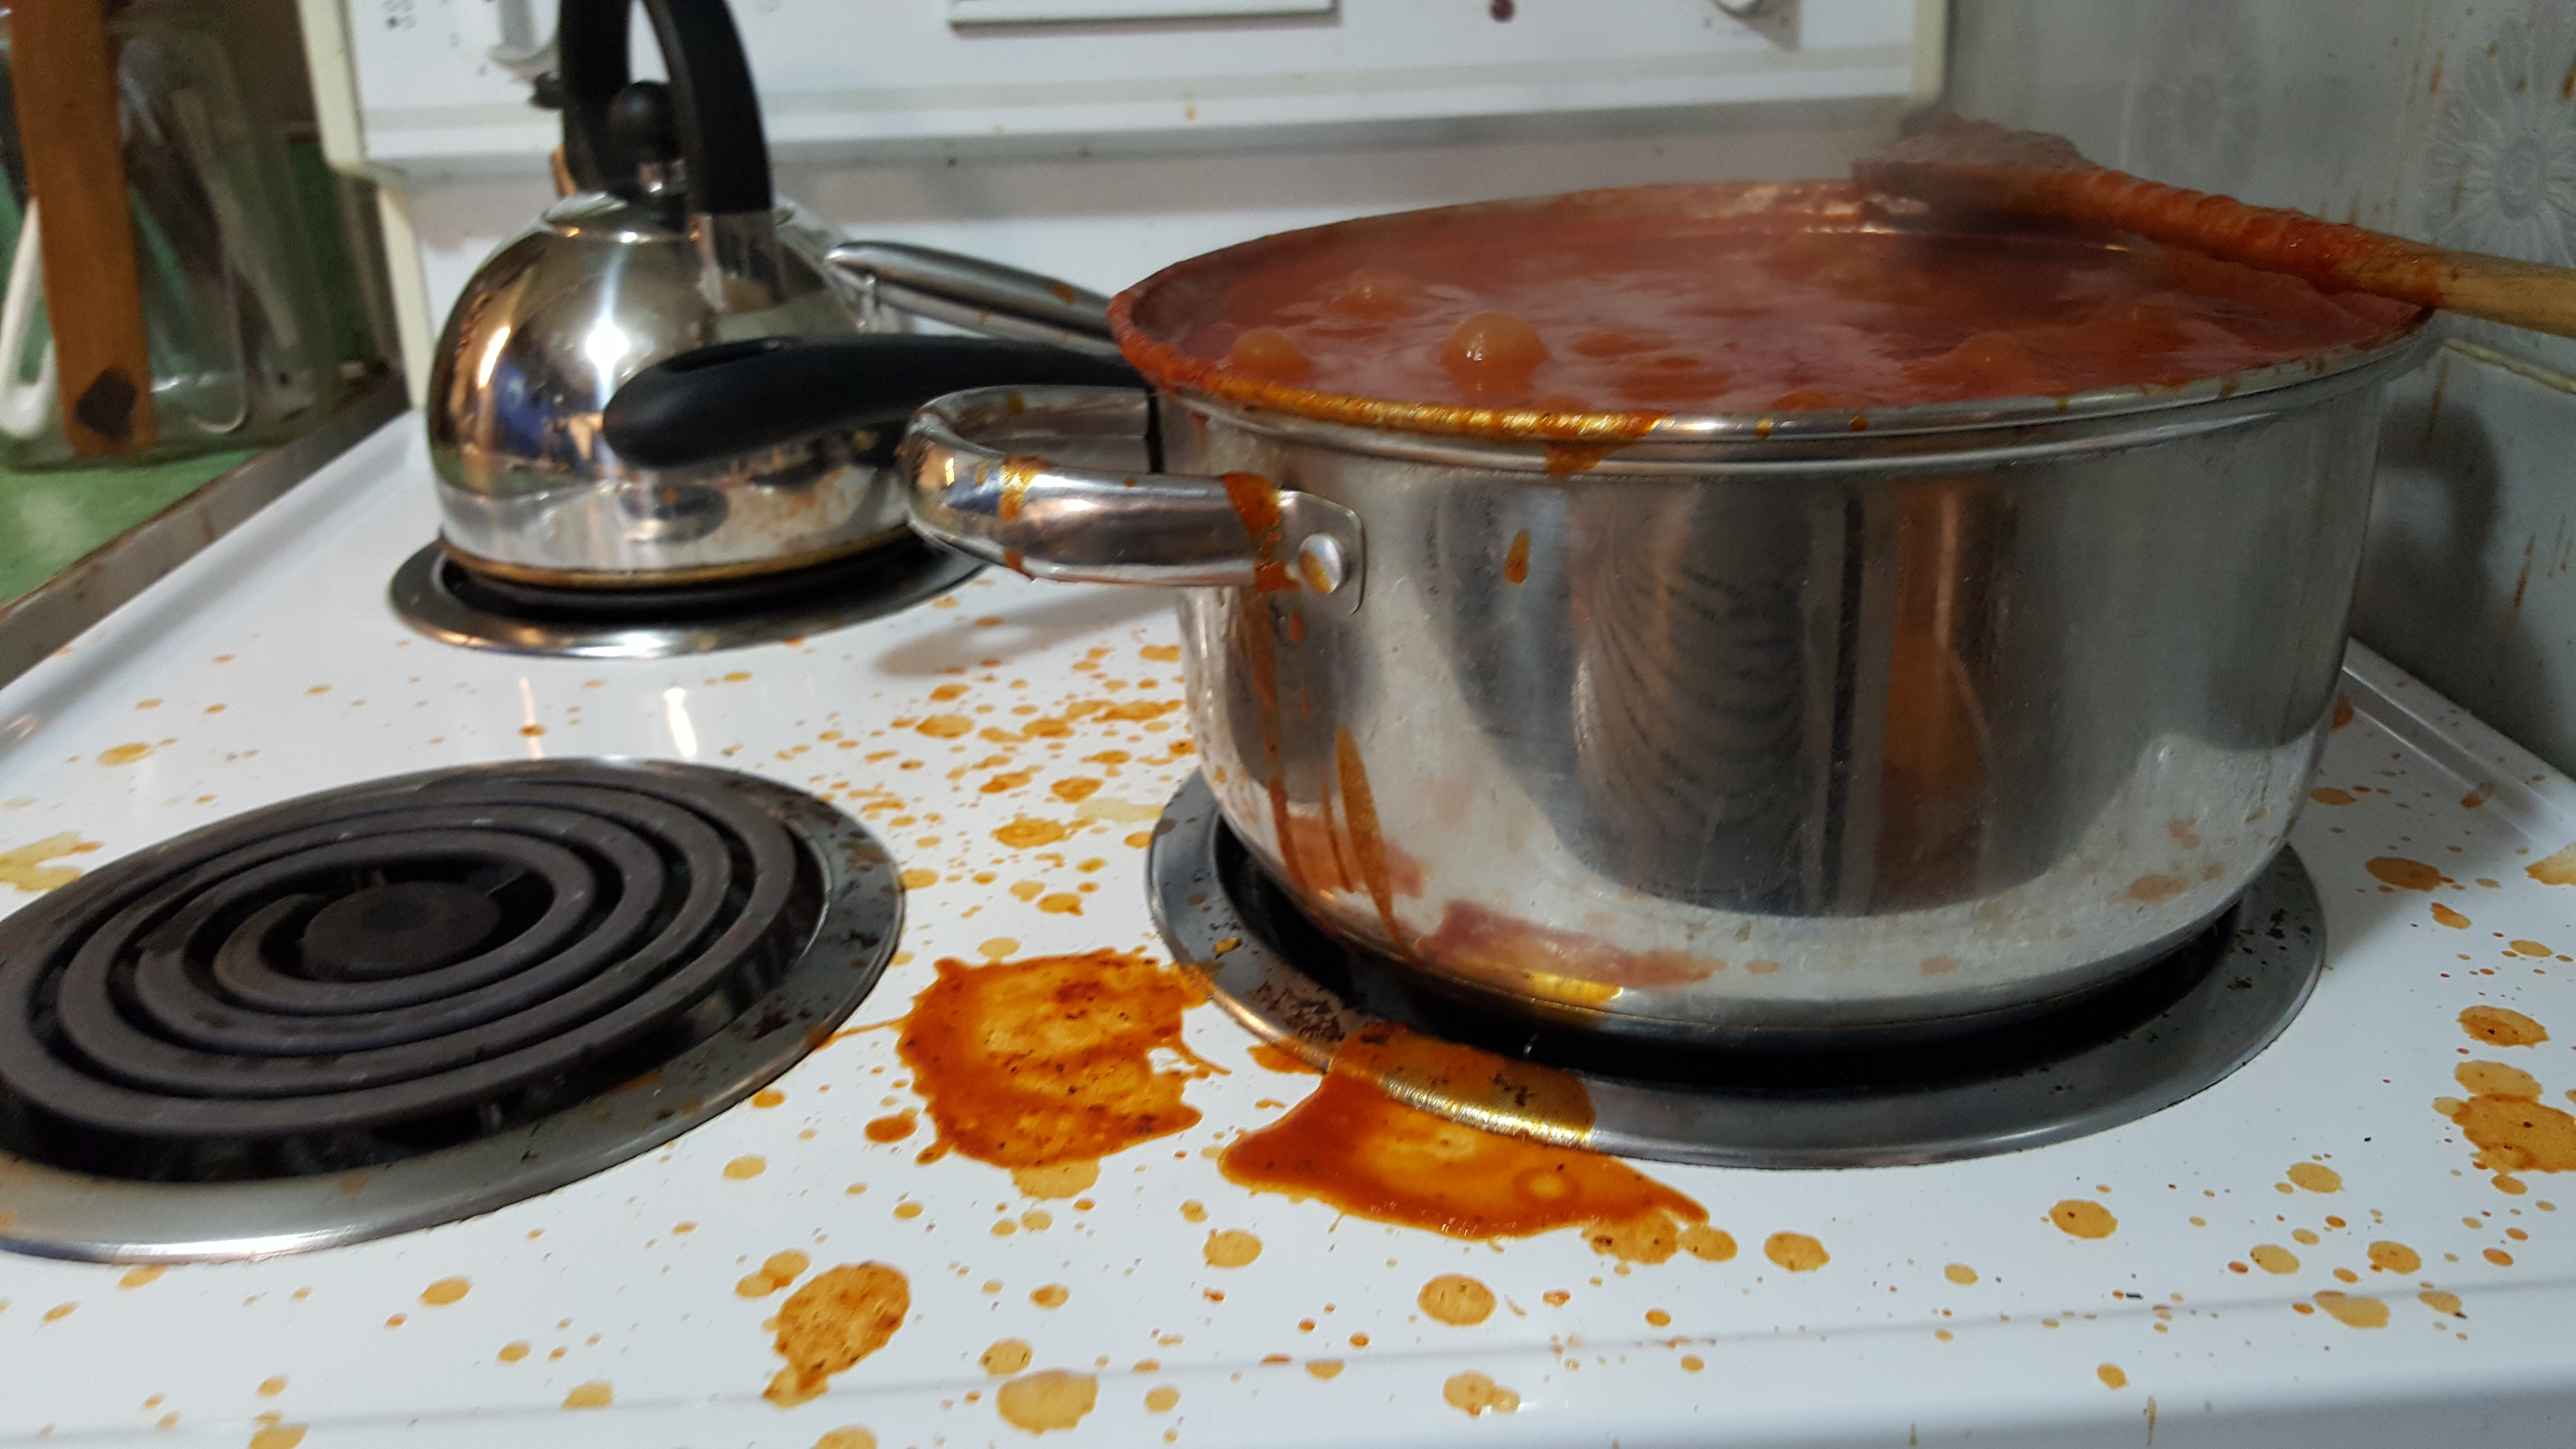
\includegraphics[trim = 1900 0 500 0, clip=true, width=\textwidth]{/home/rachel/Documents/Cookbook/Pictures/20161119_164214.jpg}
\end{figure}
\restoregeometry
\clearpage
\newpage
\newgeometry{right=0cm}



% recipe title
\section*{\fontsize{25}{15}\selectfont Tomato Sauce}
\addcontentsline{toc}{section}{Tomato Sauce}

% side figures
\begin{wrapfigure}{r}{0.5\textwidth}
\
  \begin{center}
 	\hfill\begin{minipage}{.5\textwidth}\centering
 	\vspace*{-5cm}
		\includegraphics[trim = 1100 0 1600 0, clip=true, width=0.8\textwidth]{/home/rachel/Documents/Cookbook/Pictures/20161119_161229.jpg}
		\\[5mm]
		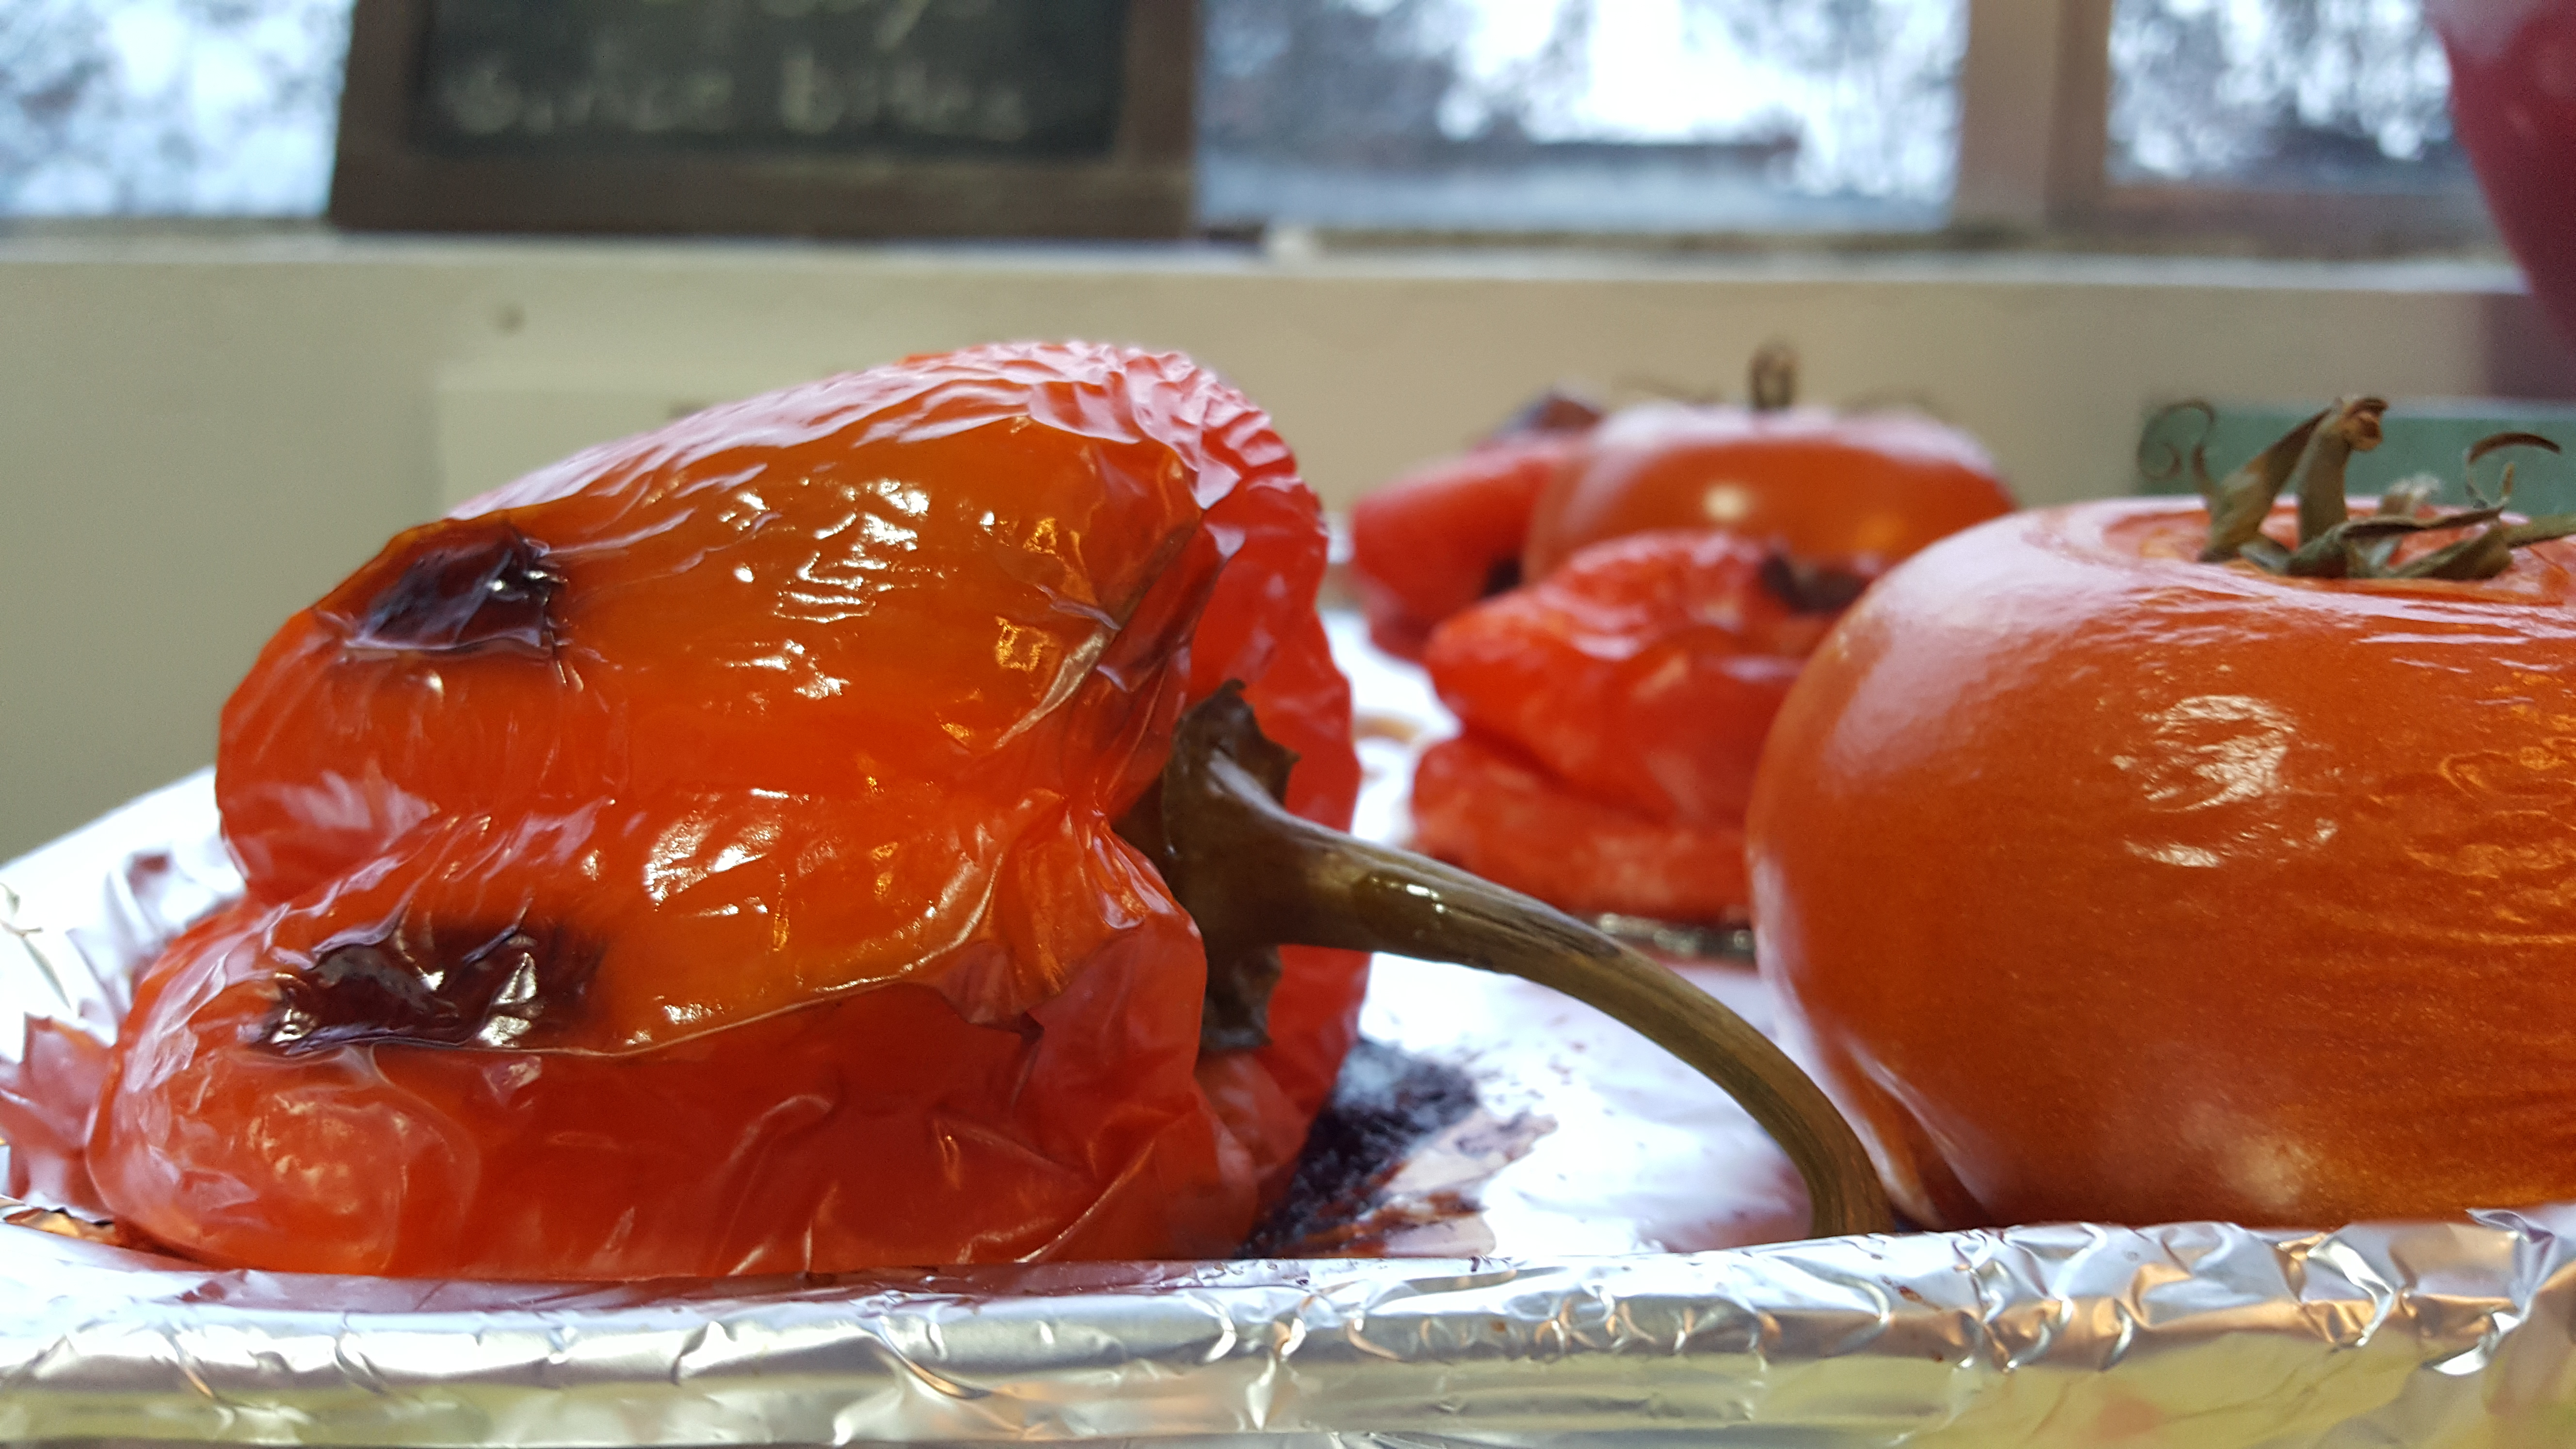
\includegraphics[trim = 0 0 200 0, clip=true, width=0.8\textwidth]{/home/rachel/Documents/Cookbook/Pictures/20161119_161220.jpg}
		\includegraphics[trim = 500 250 -200 50, clip=true, angle = -90, width=0.8\textwidth]{/home/rachel/Documents/Cookbook/Pictures/20170328_192842.jpg}
	\end{minipage}  
	\end{center}

\end{wrapfigure}



% actual recipe
\vspace{10mm}

This recipe was perfected by a Jack, but the underlying concepts that make it such a masterpiece were proposed by Rachel. This simple and straightforward recipe is sure to delight friends and mortal enemies alike. For a single batch you will need:



\vspace{5mm}
{\fontfamily{lmss}\selectfont 
    \begin{itemize}[noitemsep]
    
      \item[] 1 Jar of Ragu (I like the crunchy type myself)
      \item[] 1 Red Pepper
      \item[] 1 Green Pepper
      \item[] 2 Roma Tomatoes
      \item[] 1 Small Yellow Onion
      \item[] 2 Carrots
      \item[] Frozen Corn (As much as you want)
      \item[] Mushrooms (Optional: use as many as you want)
      \item[] 1 package of ground beef (Optional: pork works well too)
      \item[] Garlic
      \item[] Earthy Red Wine (Optional: A Malbec is a great choice)
      \item[] A Dab of Butter
      \item[] Montreal Steak Spice
      \item[] Red pepper flakes
      \item[] Italian spice (combination of oregano, basil, and salt)
      \item[] Chili Powder
      \item[] Seasoning Salt
      \item[] Pepper
      \item[] Worcestershire sauce (optional)
      
    \end{itemize}
    }


\newpage    
To produce a life changing sauce, preheat oven to 400 F, line a baking sheet with tin foil. Wash tomatoes and red pepper, and place on baking sheet roast for 1 hour, rotating every 20 minutes. Wash Mushrooms and soak in red wine, while roasting is underway brown ground beef with Worcestershire sauce and Montreal steak spice to taste, set aside (Optional)

In a separate sauce pan, bring Ragu up to gentle boil. As sauce comes to a boil add Montreal steak spice, Italian seasoning, chili powder, and red pepper flakes, and seasoning salt, and pepper to taste. Cut carrot and onions into bite sized pieces and add to sauce.Dice 1 - 3 cloves of garlic and add to sauce. Gently simmer and stir sauce as roasting finishes (this is a good time to taste the sauce to make sure it is seasoned to your taste). Slice green pepper and add to sauce as roasting concludes. Once roasted, slice tomatoes and red peppers, and add to sauce. 

Melt butter in a small pan and add mushrooms and red wine, cook on high heat until perfect. Add corn and simmer until carrots are fully cooked.

Serve mushrooms, ground beef, and sauce separately.

\restoregeometry


\settowidth{\imagewidth}{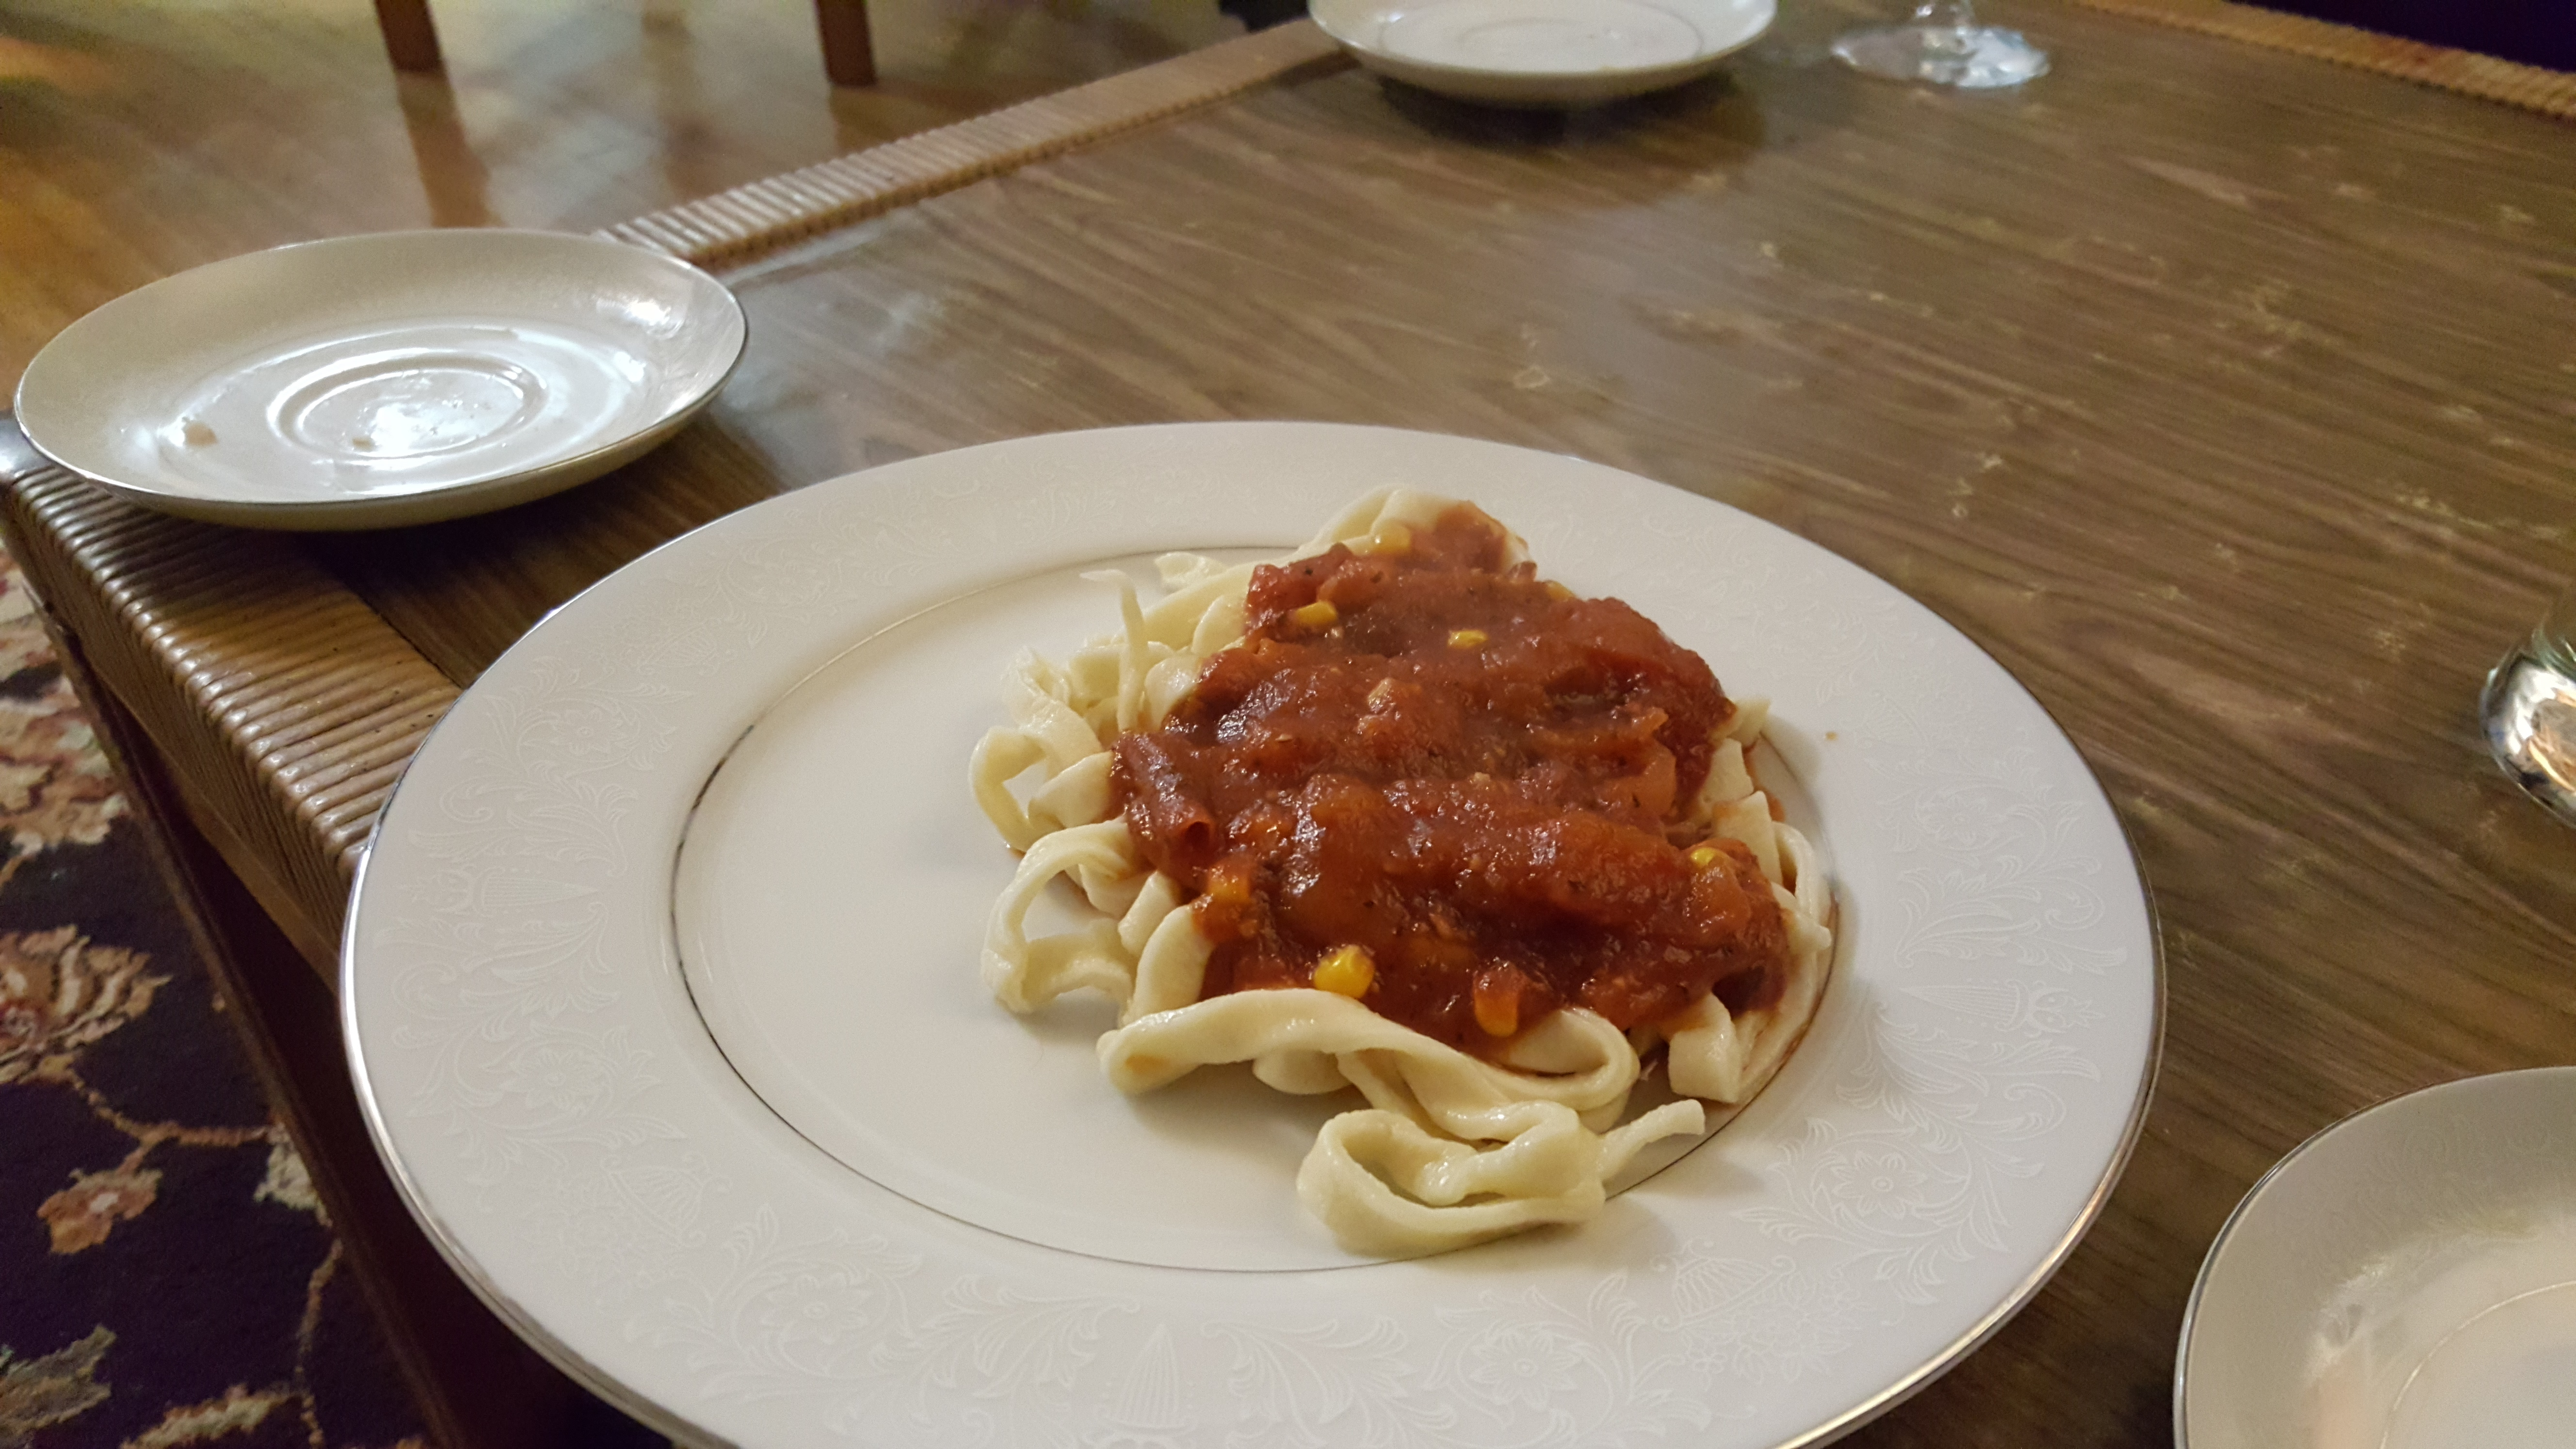
\includegraphics{/home/rachel/Documents/Cookbook/Pictures/20161119_191451.jpg}}
\newgeometry{left=0cm,bottom=0cm,top=0cm,right=0cm}
\newpage
\begin{figure}[]
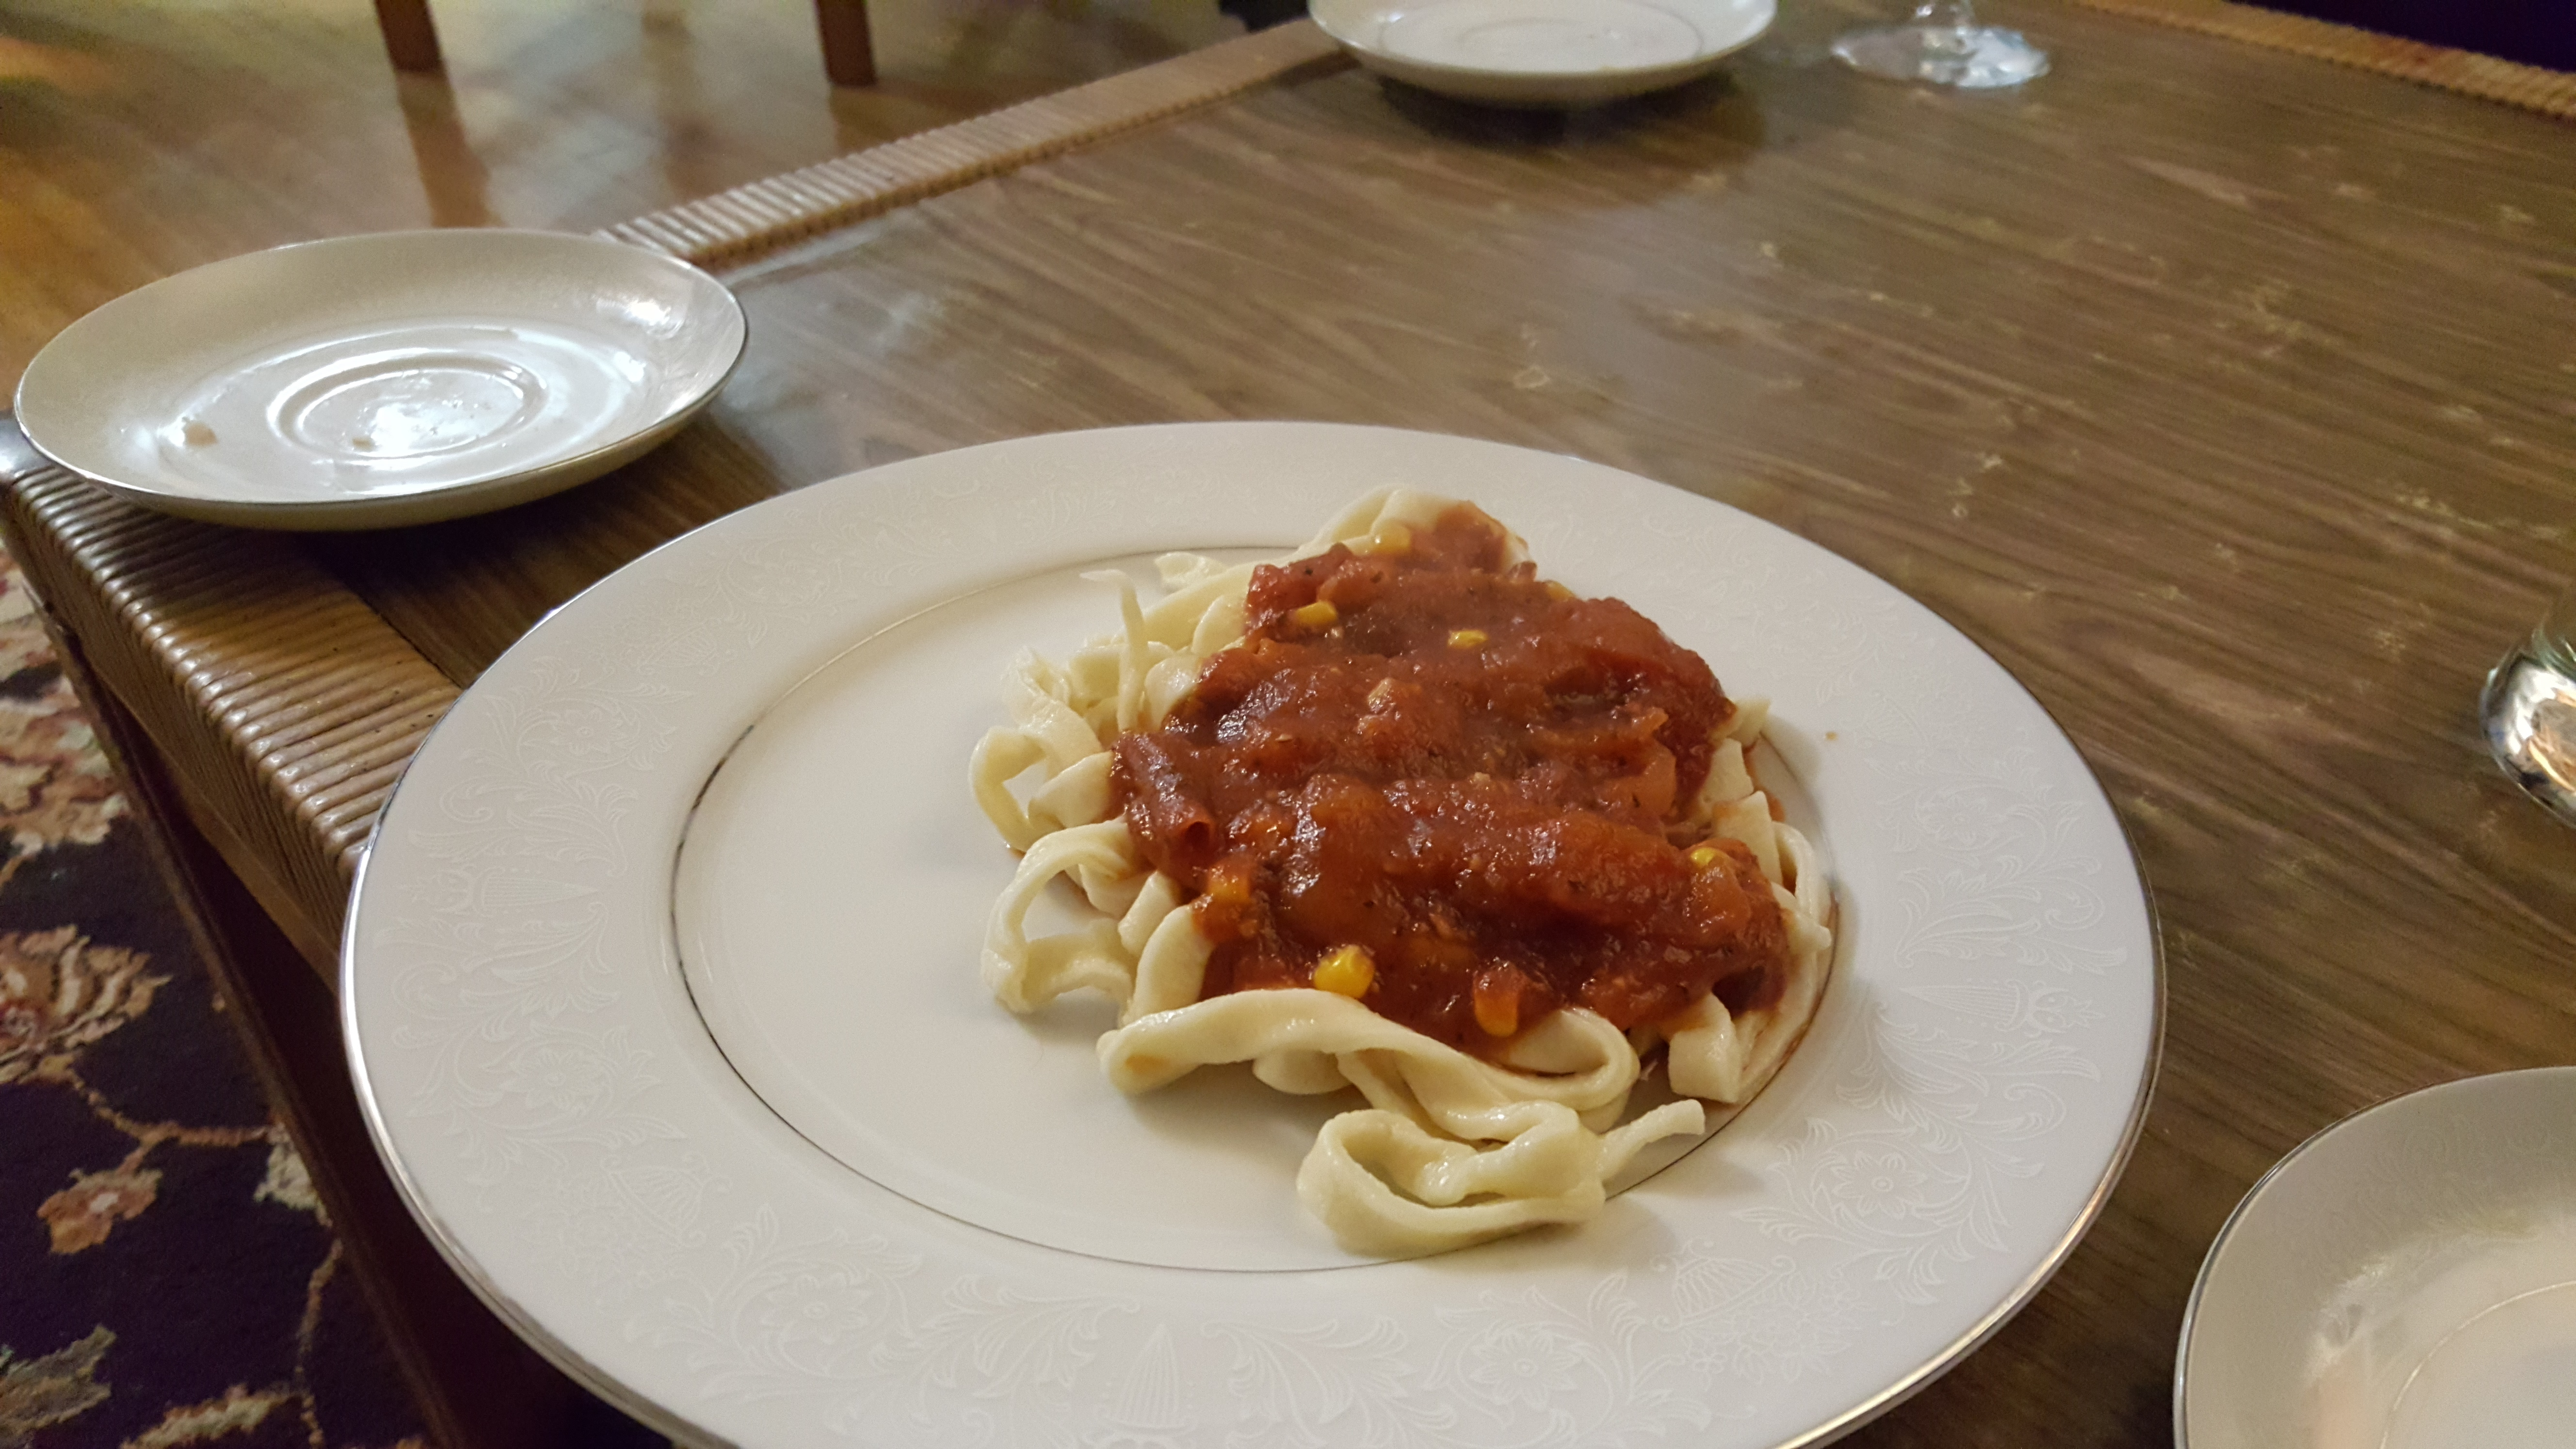
\includegraphics[trim = 1500 0 800 0, clip=true,
 width=\textwidth]{/home/rachel/Documents/Cookbook/Pictures/20161119_191451.jpg}
\end{figure}
\restoregeometry
\clearpage
\newpage
\newgeometry{right=0cm}








%%%%%%%%%%%%%%%%%%%%%%%%%%%%%%%%%%%%%%%%%%%%%%%%%%%%%%%%%%%%%%%%%%%%%%%%%%%%%%%%%%%%%%%%%%%%%%%%%%%%%%%%%%%%%%%%%%%%%%%%%%%%%%%%%%%
% Lasagna

%title picture add file name twice

\settowidth{\imagewidth}{\includegraphics{/home/rachel/Documents/Cookbook/Pictures/20160108_203228.jpg}}
\newgeometry{left=0cm,bottom=0cm,top=0cm,right=0cm}
\newpage
\begin{figure}[]
\includegraphics[trim = 0.25\imagewidth{} 0 0 0, clip=true, angle = -90, width=\textwidth]{/home/rachel/Documents/Cookbook/Pictures/20160108_203228.jpg}
\end{figure}
\restoregeometry
\clearpage
\newpage
\newgeometry{right=0cm}



% recipe title
\section*{\fontsize{25}{15}\selectfont Lasagna}
\addcontentsline{toc}{section}{Lasagna}

% side figures
\begin{wrapfigure}{r}{0.5\textwidth}
\
  \begin{center}
 	\hfill\begin{minipage}{.5\textwidth}\centering
 	\vspace*{-4.3cm}
		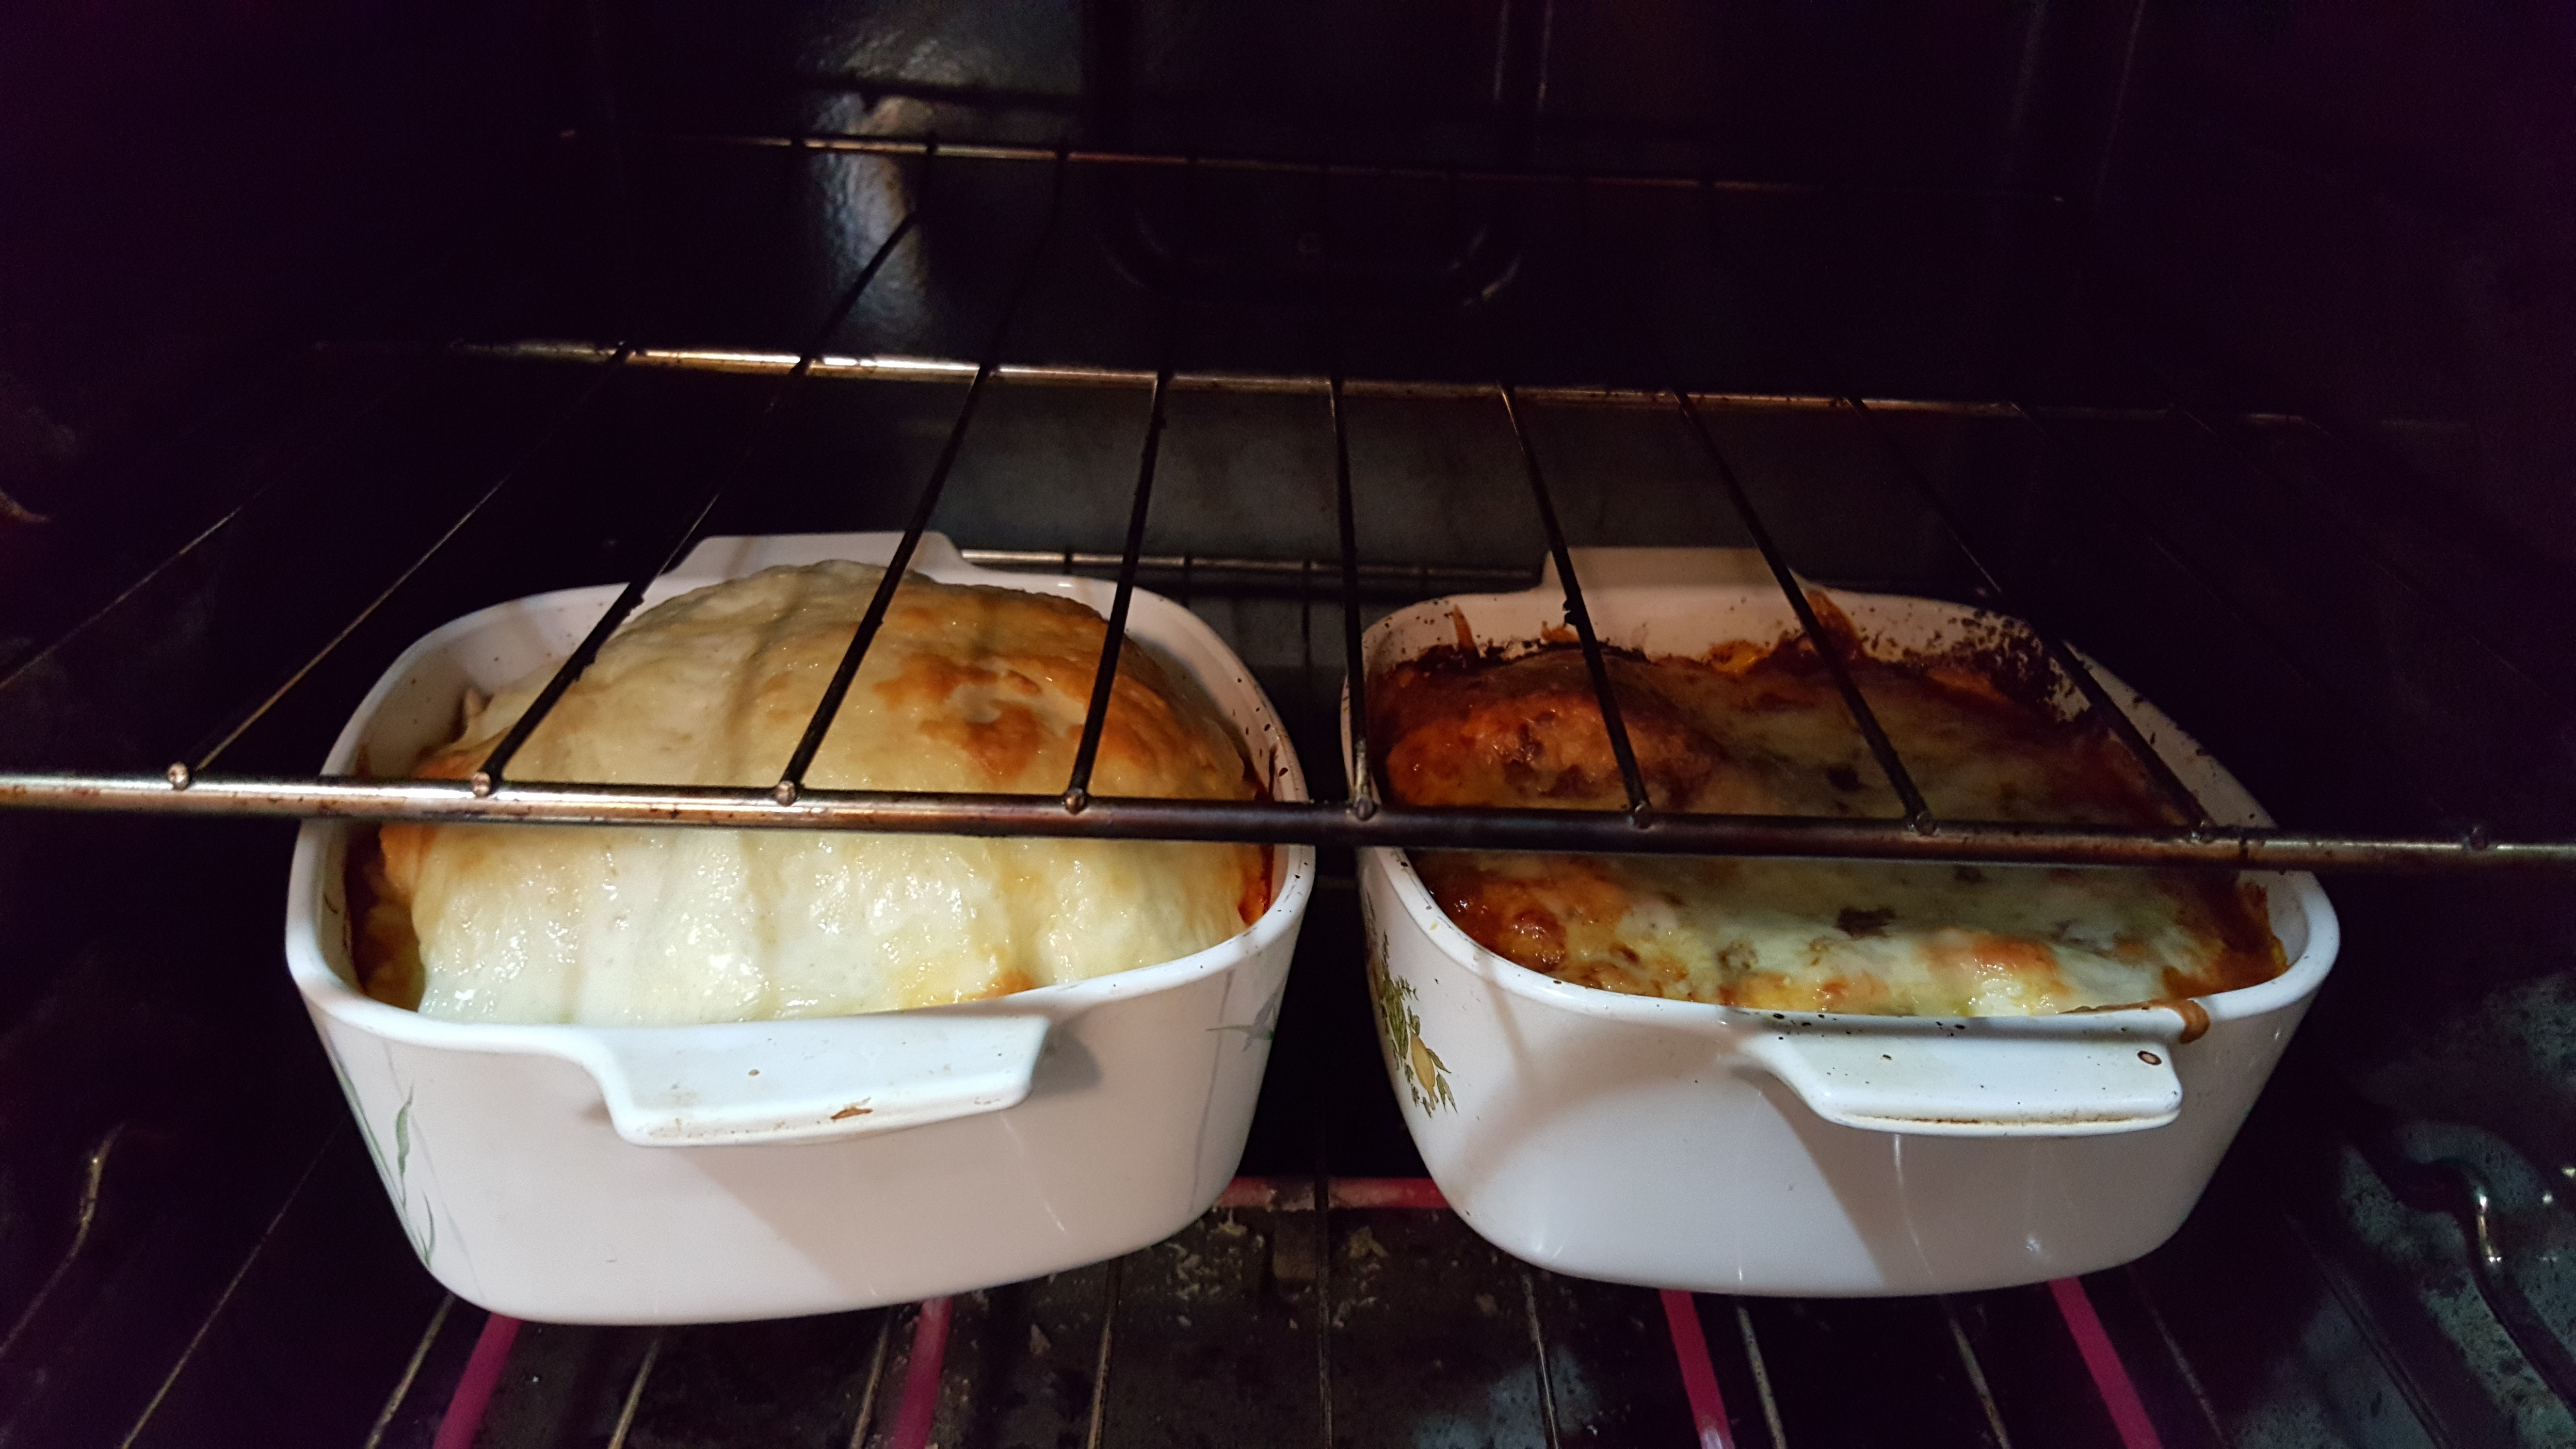
\includegraphics[trim = 0 0 0 0, clip=true, width=0.8\textwidth]{/home/rachel/Documents/Cookbook/Pictures/20160320_202125.jpg}
		\\[5mm]
		\includegraphics[trim = 0 0 0 0, clip=true,width=1.4\textwidth, angle = -90]{/home/rachel/Documents/Cookbook/Pictures/20160108_203222.jpg}
	\end{minipage}  
	\end{center}

\end{wrapfigure}



% actual recipe
\vspace{10mm}

\textbf{Need recipe}
 
\vspace{5mm}
{\fontfamily{lmss}\selectfont 
    \begin{itemize}[noitemsep]
    
      \item[] Lorem ipsum
      \item[] dolor sit
      \item[] amet
      
    \end{itemize}
    }
\vspace{5mm}
    
Nulla scelerisque efficitur arcu sed vestibulum. Donec imperdiet ipsum et placerat cursus. Quisque in mauris eu nunc malesuada bibendum. Aliquam egestas pretium dolor nec dapibus. Nulla interdum ipsum at urna ullamcorper varius. Nunc volutpat lorem sed magna vehicula lobortis. Aliquam sed scelerisque tellus. Quisque vel euismod purus, ac rhoncus nunc.

Maecenas et justo pretium, pulvinar nisl eu, facilisis urna. Etiam fermentum eros non erat porttitor pretium. Morbi efficitur, libero faucibus hendrerit accumsan, ligula tellus pulvinar erat, ac mattis odio turpis eu ex. Morbi ut justo odio. Mauris malesuada et arcu in viverra. Duis sit amet blandit quam, ac dignissim arcu. Etiam finibus pharetra felis et porttitor. Quisque felis erat, posuere nec diam quis, bibendum varius quam.

\restoregeometry








%%%%%%%%%%%%%%%%%%%%%%%%%%%%%%%%%%%%%%%%%%%%%%%%%%%%%%%%%%%%%%%%%%%%%%%%%%%%%%%%%%%%%%%%%%%%%%%%%%%%%%%%%%%%%%%%%%%%%%%%%%%%%%%%%%%
% Caesar Salad Dressing


% recipe title
\section*{\fontsize{25}{15}\selectfont Caesar Salad \\Dressing}
\addcontentsline{toc}{section}{Caesar Salad Dressing}



% side figure
\begin{wrapfigure}{r}{0.5\textwidth}
\
  \begin{center}
 	\hfill\begin{minipage}{\textwidth}\centering
 	\vspace*{-6cm}
		\includegraphics[angle=-90, trim = 750 200 0 0, width=0.8\textwidth]{/home/rachel/Documents/Cookbook/Pictures/20161125_192111.jpg}
	\end{minipage}  
	\end{center}

\end{wrapfigure}



% actual recipe
\vspace{5mm}

Jack's family dressing recipe. 
 
\vspace{5mm}
{\fontfamily{lmss}\selectfont 
    \begin{itemize}[noitemsep]
    
      \item[] 1/2 teaspoon ground pepper
      \item[] 1/2 teaspoon salt
      \item[] 1 1/2 tablespoon vinegar (cider vinegar is nice)
      \item[] 1 whole egg
      \item[] 2-3 tablespoons mayonnaise
      \item[] 2-4 cloves of garlic depending on size and personal taste
      \item[] 3/4 cup olive oil
      
    \end{itemize}
    }
\vspace{5mm}
    
Blend all of the ingredients, expect the oil, together in a blender. While the mixture is blending, slowly add the oil. Blend for 2 minutes.

\restoregeometry


%%%%%%%%%%%%%%%%%%%%%%%%%%%%%%%%%%%%%%%%%%%%%%%%%%%%%%%%%%%%%%%%%%%%%%%%%%%%%%%%%%%%%%%%%%%%%%%%%%%%%%%%%%%%%%%%%%%%%%%%%%%%%%%%%%%
% Meat Balls


% recipe title
\section*{\fontsize{25}{15}\selectfont Meat Balls}
\addcontentsline{toc}{section}{Meat Balls}
\begin{wrapfigure}{r}{0.5\textwidth}
\
  \begin{center}
 	\hfill\begin{minipage}{\textwidth}\centering
 	\vspace*{-6cm}
		\includegraphics[angle=-90, trim = 750 200 0 0, width=0.8\textwidth]{/home/rachel/Documents/Cookbook/Pictures/20160108_203251_001.jpg}
	\end{minipage}  
	\end{center}

\end{wrapfigure}



% actual recipe
\vspace{10mm}

\textbf{Need recipe}
 
\vspace{5mm}
{\fontfamily{lmss}\selectfont 
    \begin{itemize}[noitemsep]
    
      \item[] Lorem ipsum
      \item[] dolor sit
      \item[] amet
      
    \end{itemize}
    }
\vspace{5mm}
    
Nulla scelerisque efficitur arcu sed vestibulum. Donec imperdiet ipsum et placerat cursus. Quisque in mauris eu nunc malesuada bibendum. Aliquam egestas pretium dolor nec dapibus. Nulla interdum ipsum at urna ullamcorper varius. Nunc volutpat lorem sed magna vehicula lobortis. Aliquam sed scelerisque tellus. Quisque vel euismod purus, ac rhoncus nunc.

Maecenas et justo pretium, pulvinar nisl eu, facilisis urna. Etiam fermentum eros non erat porttitor pretium. Morbi efficitur, libero faucibus hendrerit accumsan, ligula tellus pulvinar erat, ac mattis odio turpis eu ex. Morbi ut justo odio. Mauris malesuada et arcu in viverra. Duis sit amet blandit quam, ac dignissim arcu. Etiam finibus pharetra felis et porttitor. Quisque felis erat, posuere nec diam quis, bibendum varius quam.

\restoregeometry





%%%%%%%%%%%%%%%%%%%%%%%%%%%%%%%%%%%%%%%%%%%%%%%%%%%%%%%%%%%%%%%%%%%%%%%%%%%%%%%%%%%%%%%%%%%%%%%%%%%%%%%%%%%%%%%%%%%%%%%%%%%%%%%%%%%
% Fully Loaded Nachos

%title picture add file name twice

\settowidth{\imagewidth}{\includegraphics{/home/rachel/Documents/Cookbook/Pictures/20161126_184847.jpg}}
\newgeometry{left=0cm,bottom=0cm,top=0cm,right=0cm}
\newpage
\begin{figure}[]
\includegraphics[trim = 1500 0 0 0, angle=-90, clip=true, width=\textwidth]{/home/rachel/Documents/Cookbook/Pictures/20161126_184847.jpg}
\end{figure}
\restoregeometry
\clearpage
\newpage
\newgeometry{right=0cm}



% recipe title
\section*{ \fontsize{25}{15}\selectfont Fully Loaded Nachos}
\addcontentsline{toc}{section}{Fully Loaded Nachos}



% side figures
\begin{wrapfigure}{r}{0.5\textwidth}
\
  \begin{center}
 	\hfill\begin{minipage}{.5\textwidth}\centering
 	\vspace*{-6cm}
		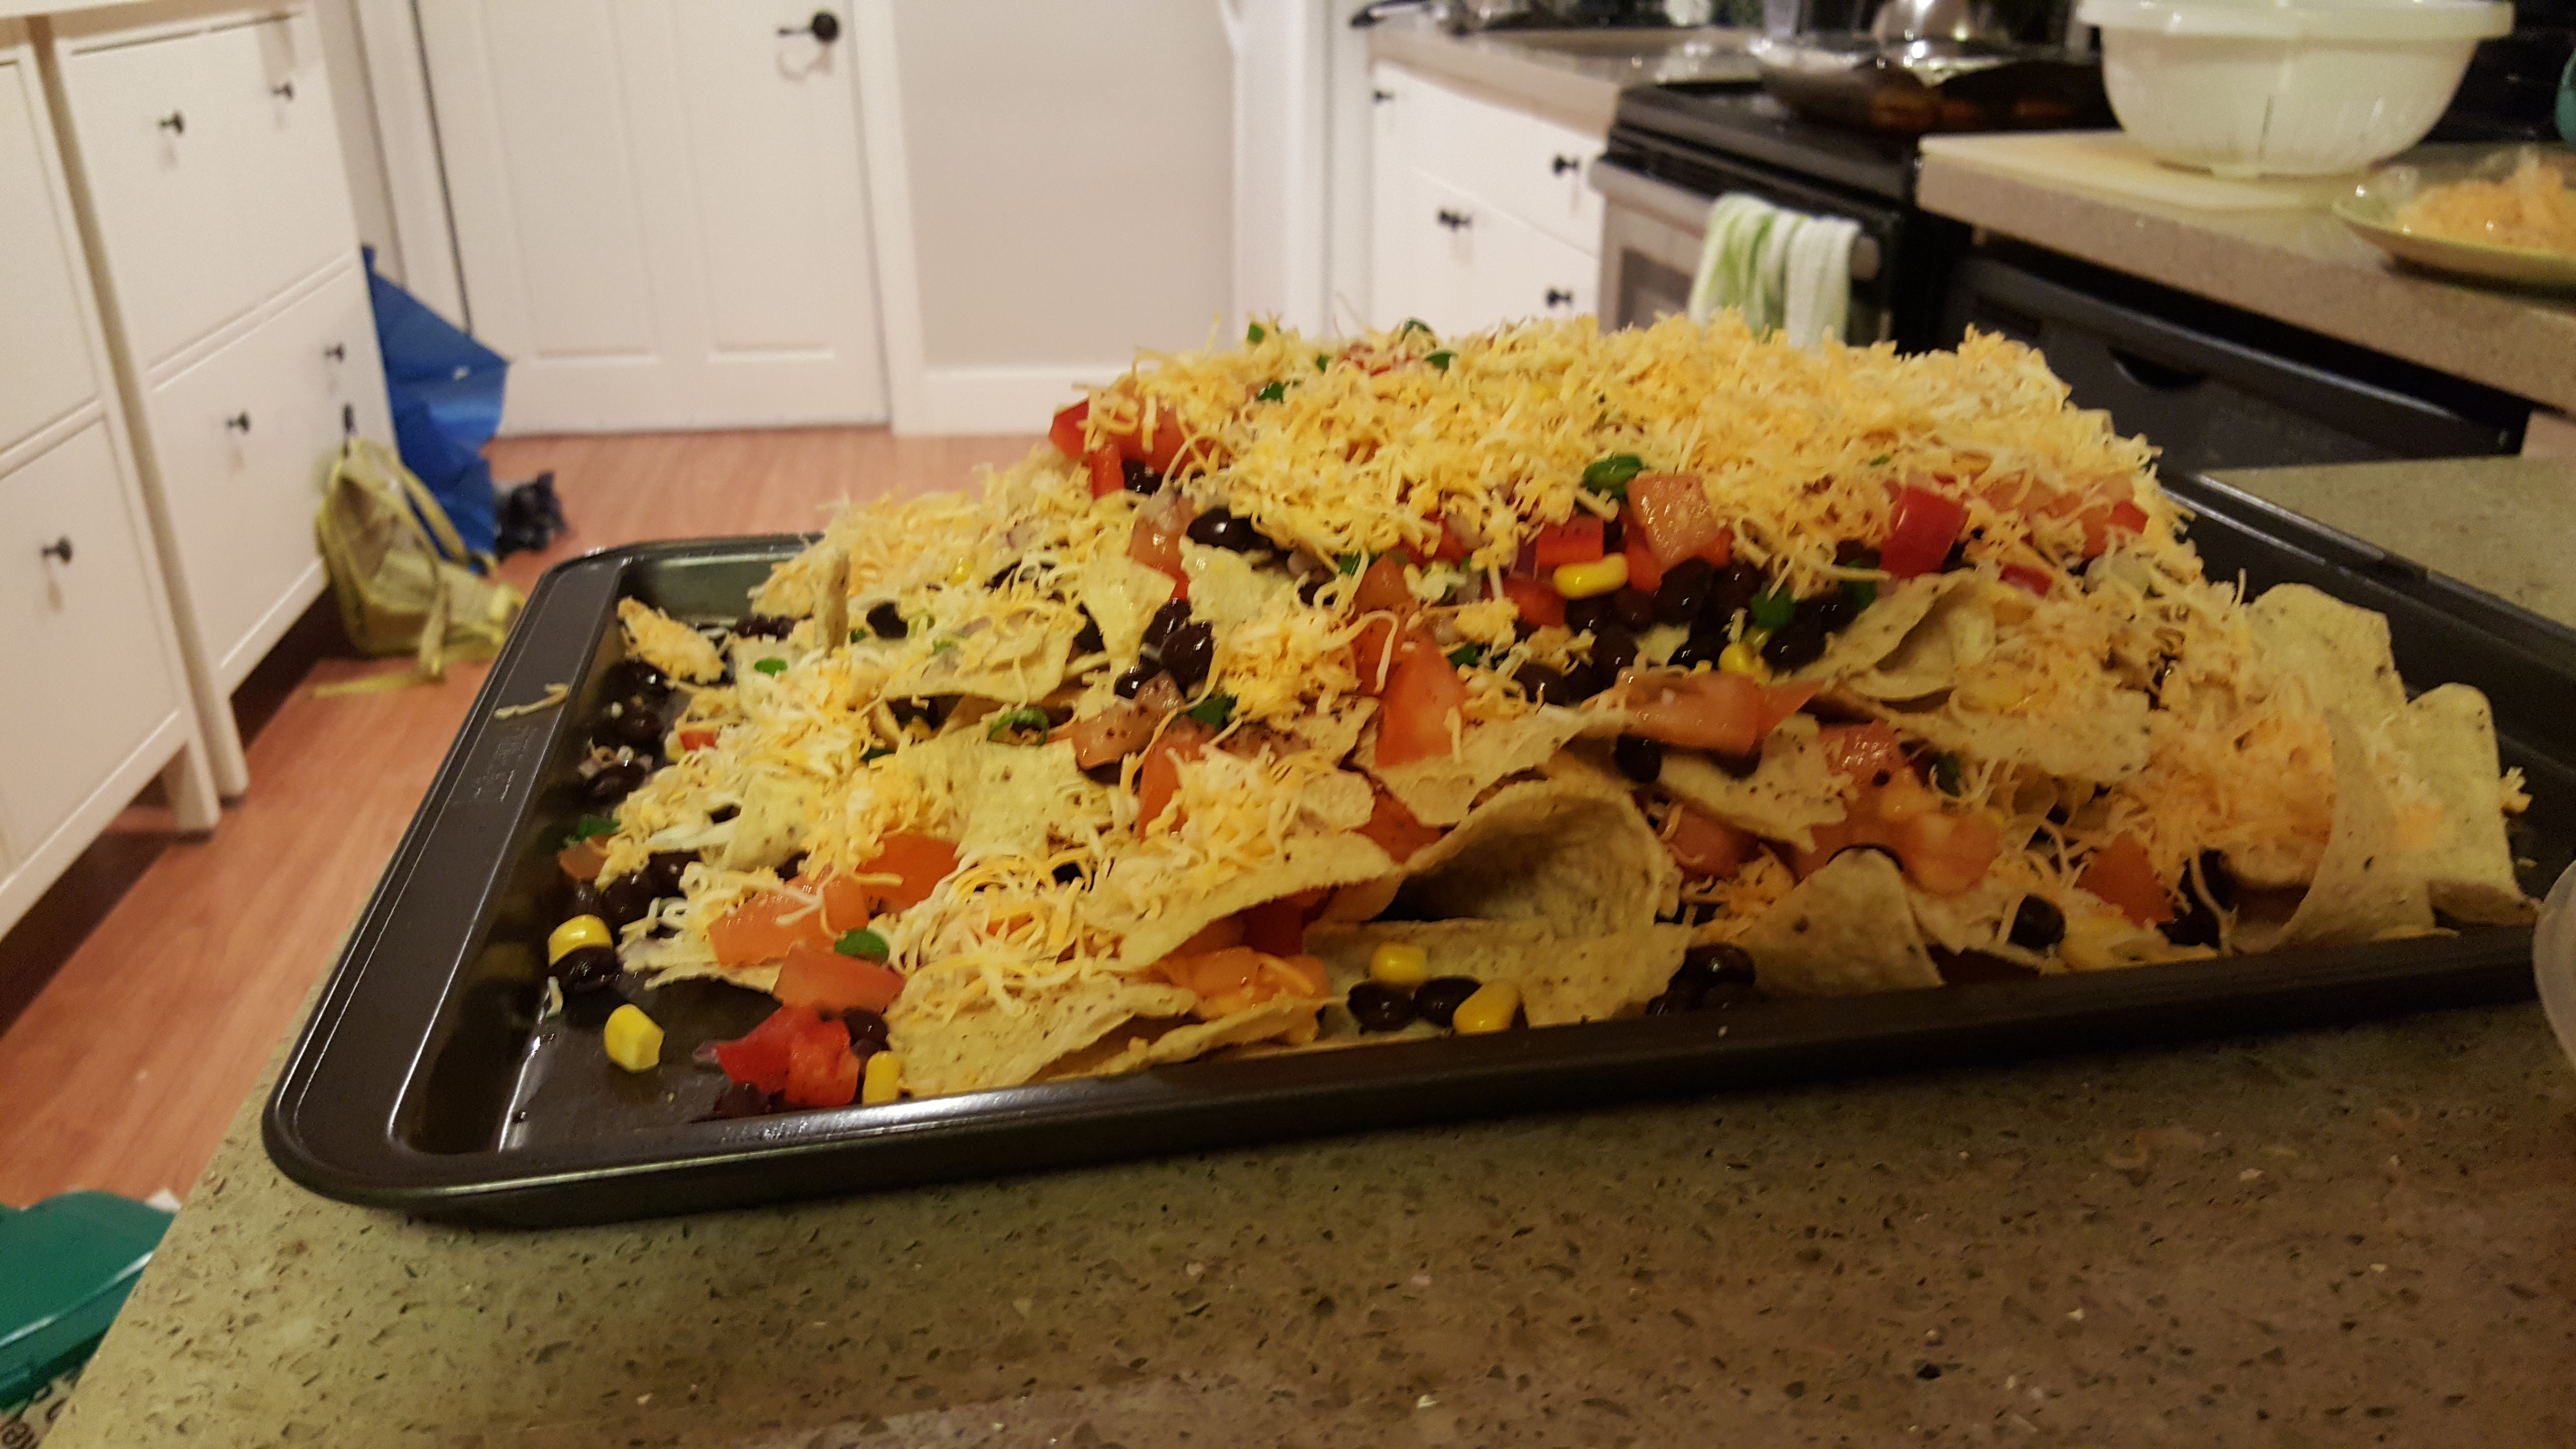
\includegraphics[trim=500 0 1300 0, clip=true, width=0.8\textwidth]{/home/rachel/Documents/Cookbook/Pictures/20161126_183746.jpg}
		\\[5mm]
		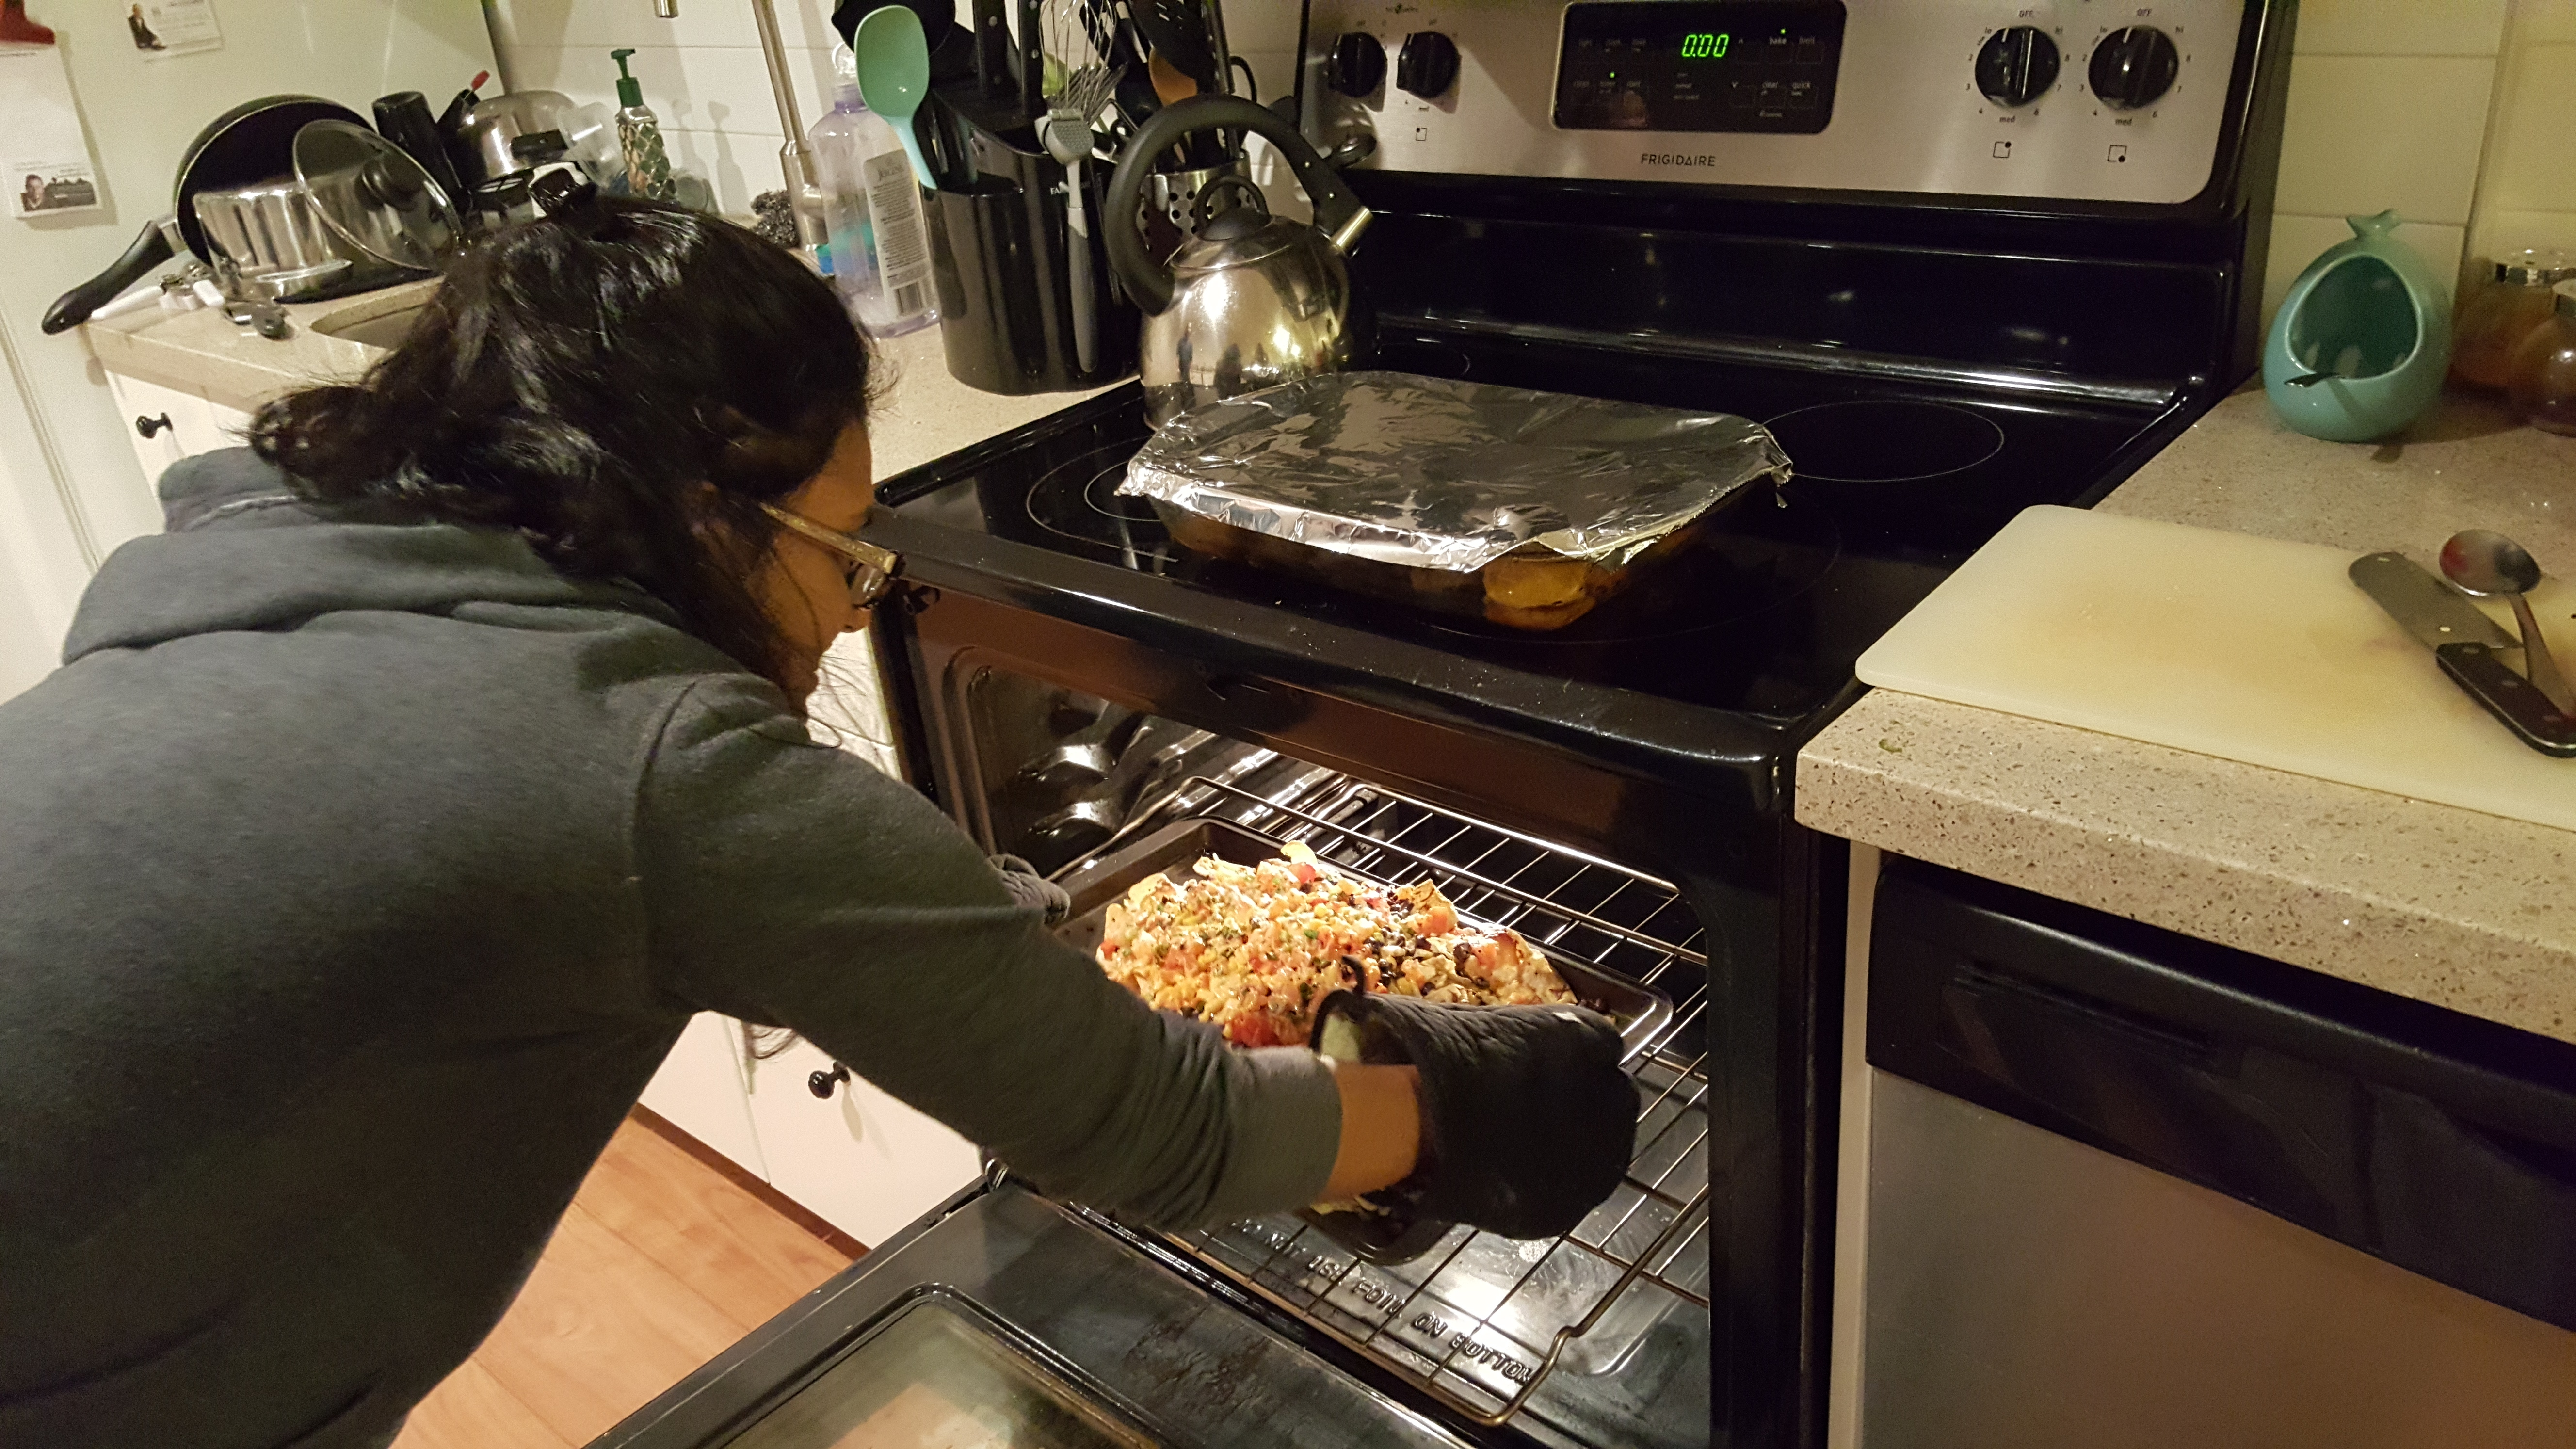
\includegraphics[trim=500 0 1300 0, clip=true,width=0.8\textwidth]{/home/rachel/Documents/Cookbook/Pictures/20161126_184828.jpg}
		\\[5mm]
		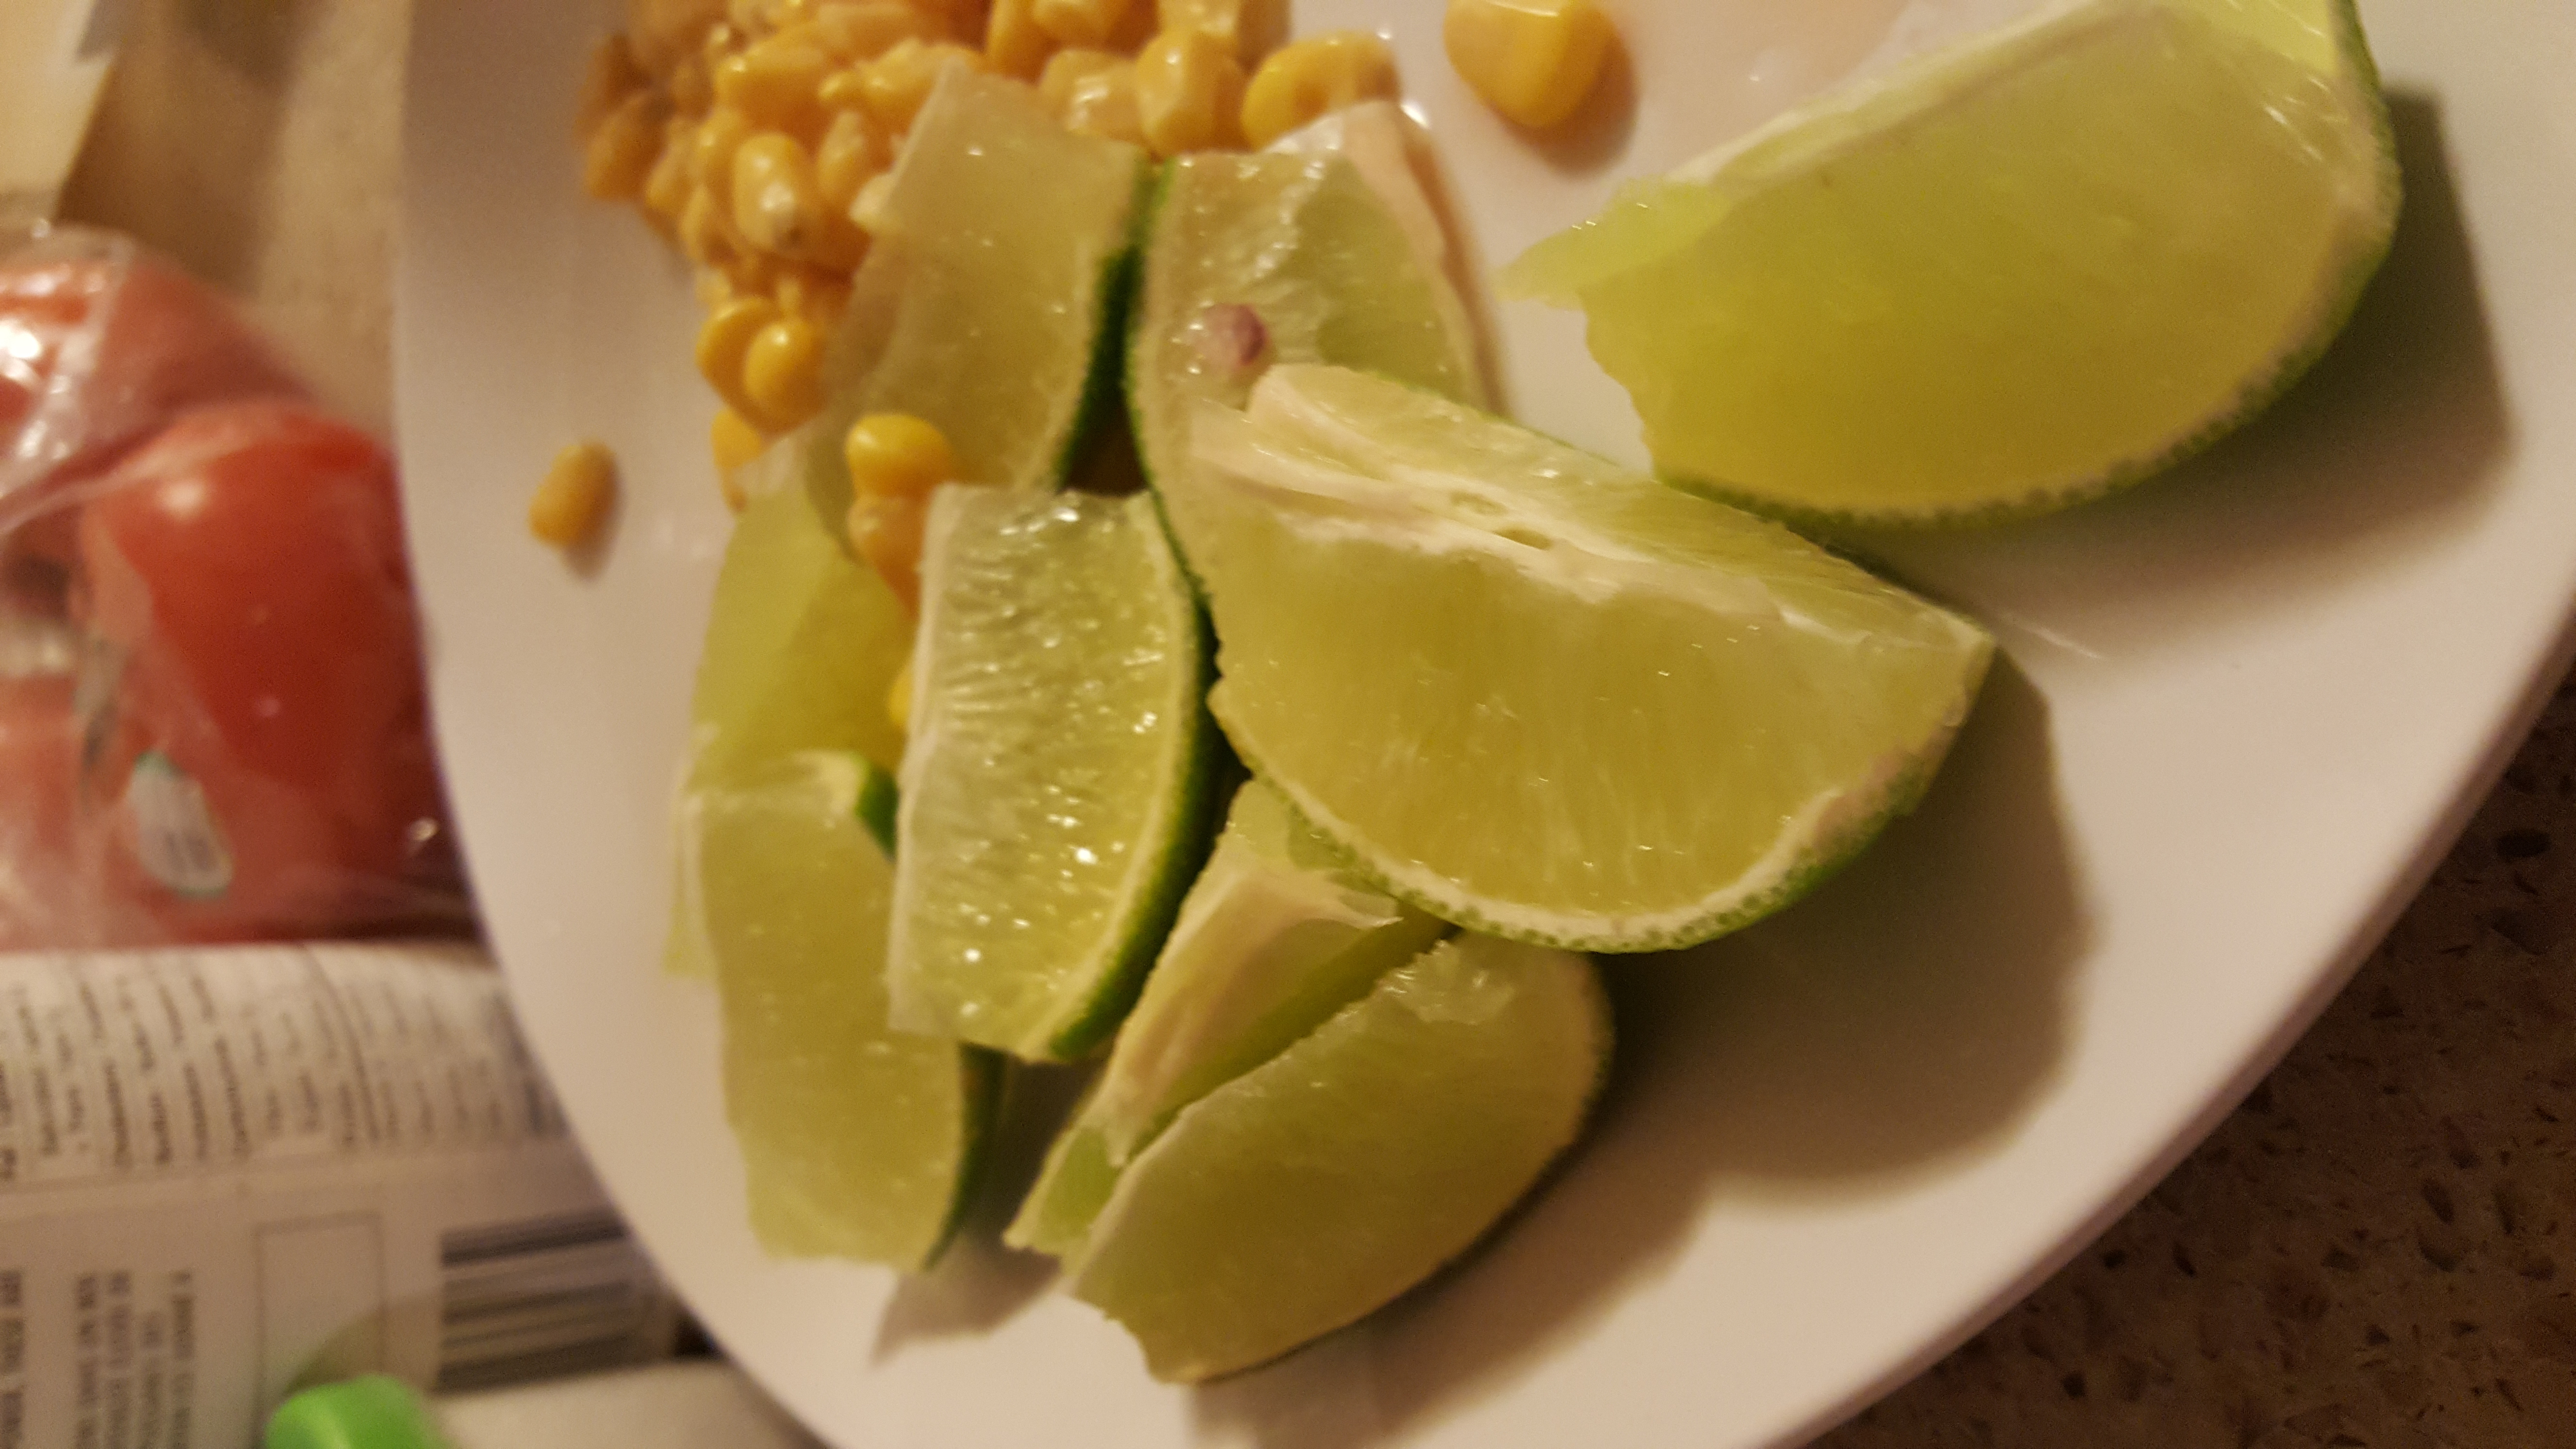
\includegraphics[trim = 800 0 0 0, angle=-90, clip=true, width=0.8\textwidth]{/home/rachel/Documents/Cookbook/Pictures/20161126_183728.jpg}

	\end{minipage}  
	\end{center}

\end{wrapfigure}


% actual recipe
\vspace{10mm}

Feast on a mountain of nacho, layers on layers of toppings. Definitely a full meal on it's own,but also possible to have tacos after.
 
\vspace{5mm}
{\fontfamily{lmss}\selectfont 
    \begin{itemize}[noitemsep]
    
      \item[] Corn chips
      \item[] Cheddar cheese (you decide how much, you are a responsible adult)
      \item[] Black beans (cooked or from a can)
      \item[] Chopped bell pepper
      \item[] Corn
      \item[] Spicy pepper
      \item[] Tomato
      \item[] Green onion
      \item[] 1 tsp chili powder 
      \item[] Lime
      
    \end{itemize}
    }
\vspace{5mm}
    
Pre-heat oven to 400\degree F. Oil cookie sheet and spread half the chips onto the sheet. Top with have the toppings and half the chili powder. Then added the remaining chips and toppings. Bake for 8-10 minutes. Top with lime juice.

\restoregeometry



%%%%%%%%%%%%%%%%%%%%%%%%%%%%%%%%%%%%%%%%%%%%%%%%%%%%%%%%%%%%%%%%%%%%%%%%%%%%%%%%%%%%%%%%%%%%%%%%%%%%%%%%%%%%%%%%%%%%%%%%%%%%%%%%%%%
% Guacamole


% recipe title
\section*{\fontsize{25}{15}\selectfont Guacamole}
\addcontentsline{toc}{section}{Guacamole}



% side figure
\begin{wrapfigure}{r}{0.5\textwidth}
\
  \begin{center}
 	\hfill\begin{minipage}{\textwidth}\centering
 	\vspace*{-6cm}
		\includegraphics[angle=-90, trim = 0 0 0 0, width=0.8\textwidth]{/home/rachel/Documents/Cookbook/Pictures/placeholder.png}
	\end{minipage}  
	\end{center}

\end{wrapfigure}



% actual recipe
\vspace{5mm}

So fresh and delicious, cuts the heat from the other taco night stuff.
 
\vspace{5mm}
{\fontfamily{lmss}\selectfont 
    \begin{itemize}[noitemsep]
    
      \item[] 2 avocados
      \item[] 1-2 tbsp finely chopped cilantro
      \item[] 1 roma tomato
      \item[] 1/4 onion
      \item[] juice of 1/2 a lime
      \item[] salt and pepper
           
    \end{itemize}
    }
\vspace{5mm}
    
Mash the avocado in a bowl with a fork. Add cilantro, tomato, onion, and lime juice. Salt and pepper to taste.

\textit{ Tip adding the pit of one avocado to the guacamole and then sealing the exposed part of the guacamole with plastic wrap will minimize the oxidation and browning.}

\restoregeometry

%%%%%%%%%%%%%%%%%%%%%%%%%%%%%%%%%%%%%%%%%%%%%%%%%%%%%%%%%%%%%%%%%%%%%%%%%%%%%%%%%%%%%%%%%%%%%%%%%%%%%%%%%%%%%%%%%%%%%%%%%%%%%%%%%%%
% Beef Carnitas


% recipe title
\section*{\fontsize{25}{15}\selectfont Beef Carnitas}
\addcontentsline{toc}{section}{Beef Carnitas}



% side figure
\begin{wrapfigure}{r}{0.5\textwidth}
\
  \begin{center}
 	\hfill\begin{minipage}{\textwidth}\centering
 	\vspace*{-6cm}
		\includegraphics[trim = 400 0 0 0, angle=-90, clip=true,width=0.6\textwidth]{/home/rachel/Documents/Cookbook/Pictures/IMG-20161126-WA00002.jpg}
	\end{minipage}  
	\end{center}

\end{wrapfigure}



% actual recipe
\vspace{5mm}

\textbf{Need recipe}
 
\vspace{5mm}
{\fontfamily{lmss}\selectfont 
    \begin{itemize}[noitemsep]
    
      \item[] 1/2 teaspoon ground pepper
      \item[] 1/2 teaspoon salt
      \item[] 1 1/2 tablespoon vinegar (cider vinegar is nice)
      \item[] 1 whole egg
      \item[] 2-3 tablespoons mayonnaise
      \item[] 2-4 cloves of garlic depending on size and personal taste
      \item[] 3/4 cup olive oil
      
    \end{itemize}
    }
\vspace{5mm}
    
Blend all of the ingredients, expect the oil, together in a blender. While the mixture is blending, slowly add the oil. Blend for 2 minutes.

\restoregeometry

%%%%%%%%%%%%%%%%%%%%%%%%%%%%%%%%%%%%%%%%%%%%%%%%%%%%%%%%%%%%%%%%%%%%%%%%%%%%%%%%%%%%%%%%%%%%%%%%%%%%%%%%%%%%%%%%%%%%%%%%%%%%%%%%%%%
% Sumaiyas Chicken


% recipe title
\section*{\fontsize{25}{15}\selectfont Sumaiyas Chicken}
\addcontentsline{toc}{section}{Sumaiyas Chicken}



% side figure
\begin{wrapfigure}{r}{0.5\textwidth}
\
  \begin{center}
 	\hfill\begin{minipage}{\textwidth}\centering
 	\vspace*{-6cm}
		\includegraphics[angle=-90, trim = 0 0 0 0, width=0.8\textwidth]{/home/rachel/Documents/Cookbook/Pictures/placeholder.png}
	\end{minipage}  
	\end{center}

\end{wrapfigure}



% actual recipe
\vspace{5mm}

\textbf{Need recipe}
 
\vspace{5mm}
{\fontfamily{lmss}\selectfont 
    \begin{itemize}[noitemsep]
    
      \item[] 1/2 teaspoon ground pepper
      \item[] 1/2 teaspoon salt
      \item[] 1 1/2 tablespoon vinegar (cider vinegar is nice)
      \item[] 1 whole egg
      \item[] 2-3 tablespoons mayonnaise
      \item[] 2-4 cloves of garlic depending on size and personal taste
      \item[] 3/4 cup olive oil
      
    \end{itemize}
    }
\vspace{5mm}
    
Blend all of the ingredients, expect the oil, together in a blender. While the mixture is blending, slowly add the oil. Blend for 2 minutes.

\restoregeometry

%%%%%%%%%%%%%%%%%%%%%%%%%%%%%%%%%%%%%%%%%%%%%%%%%%%%%%%%%%%%%%%%%%%%%%%%%%%%%%%%%%%%%%%%%%%%%%%%%%%%%%%%%%%%%%%%%%%%%%%%%%%%%%%%%%%
% Taco Toppings


\settowidth{\imagewidth}{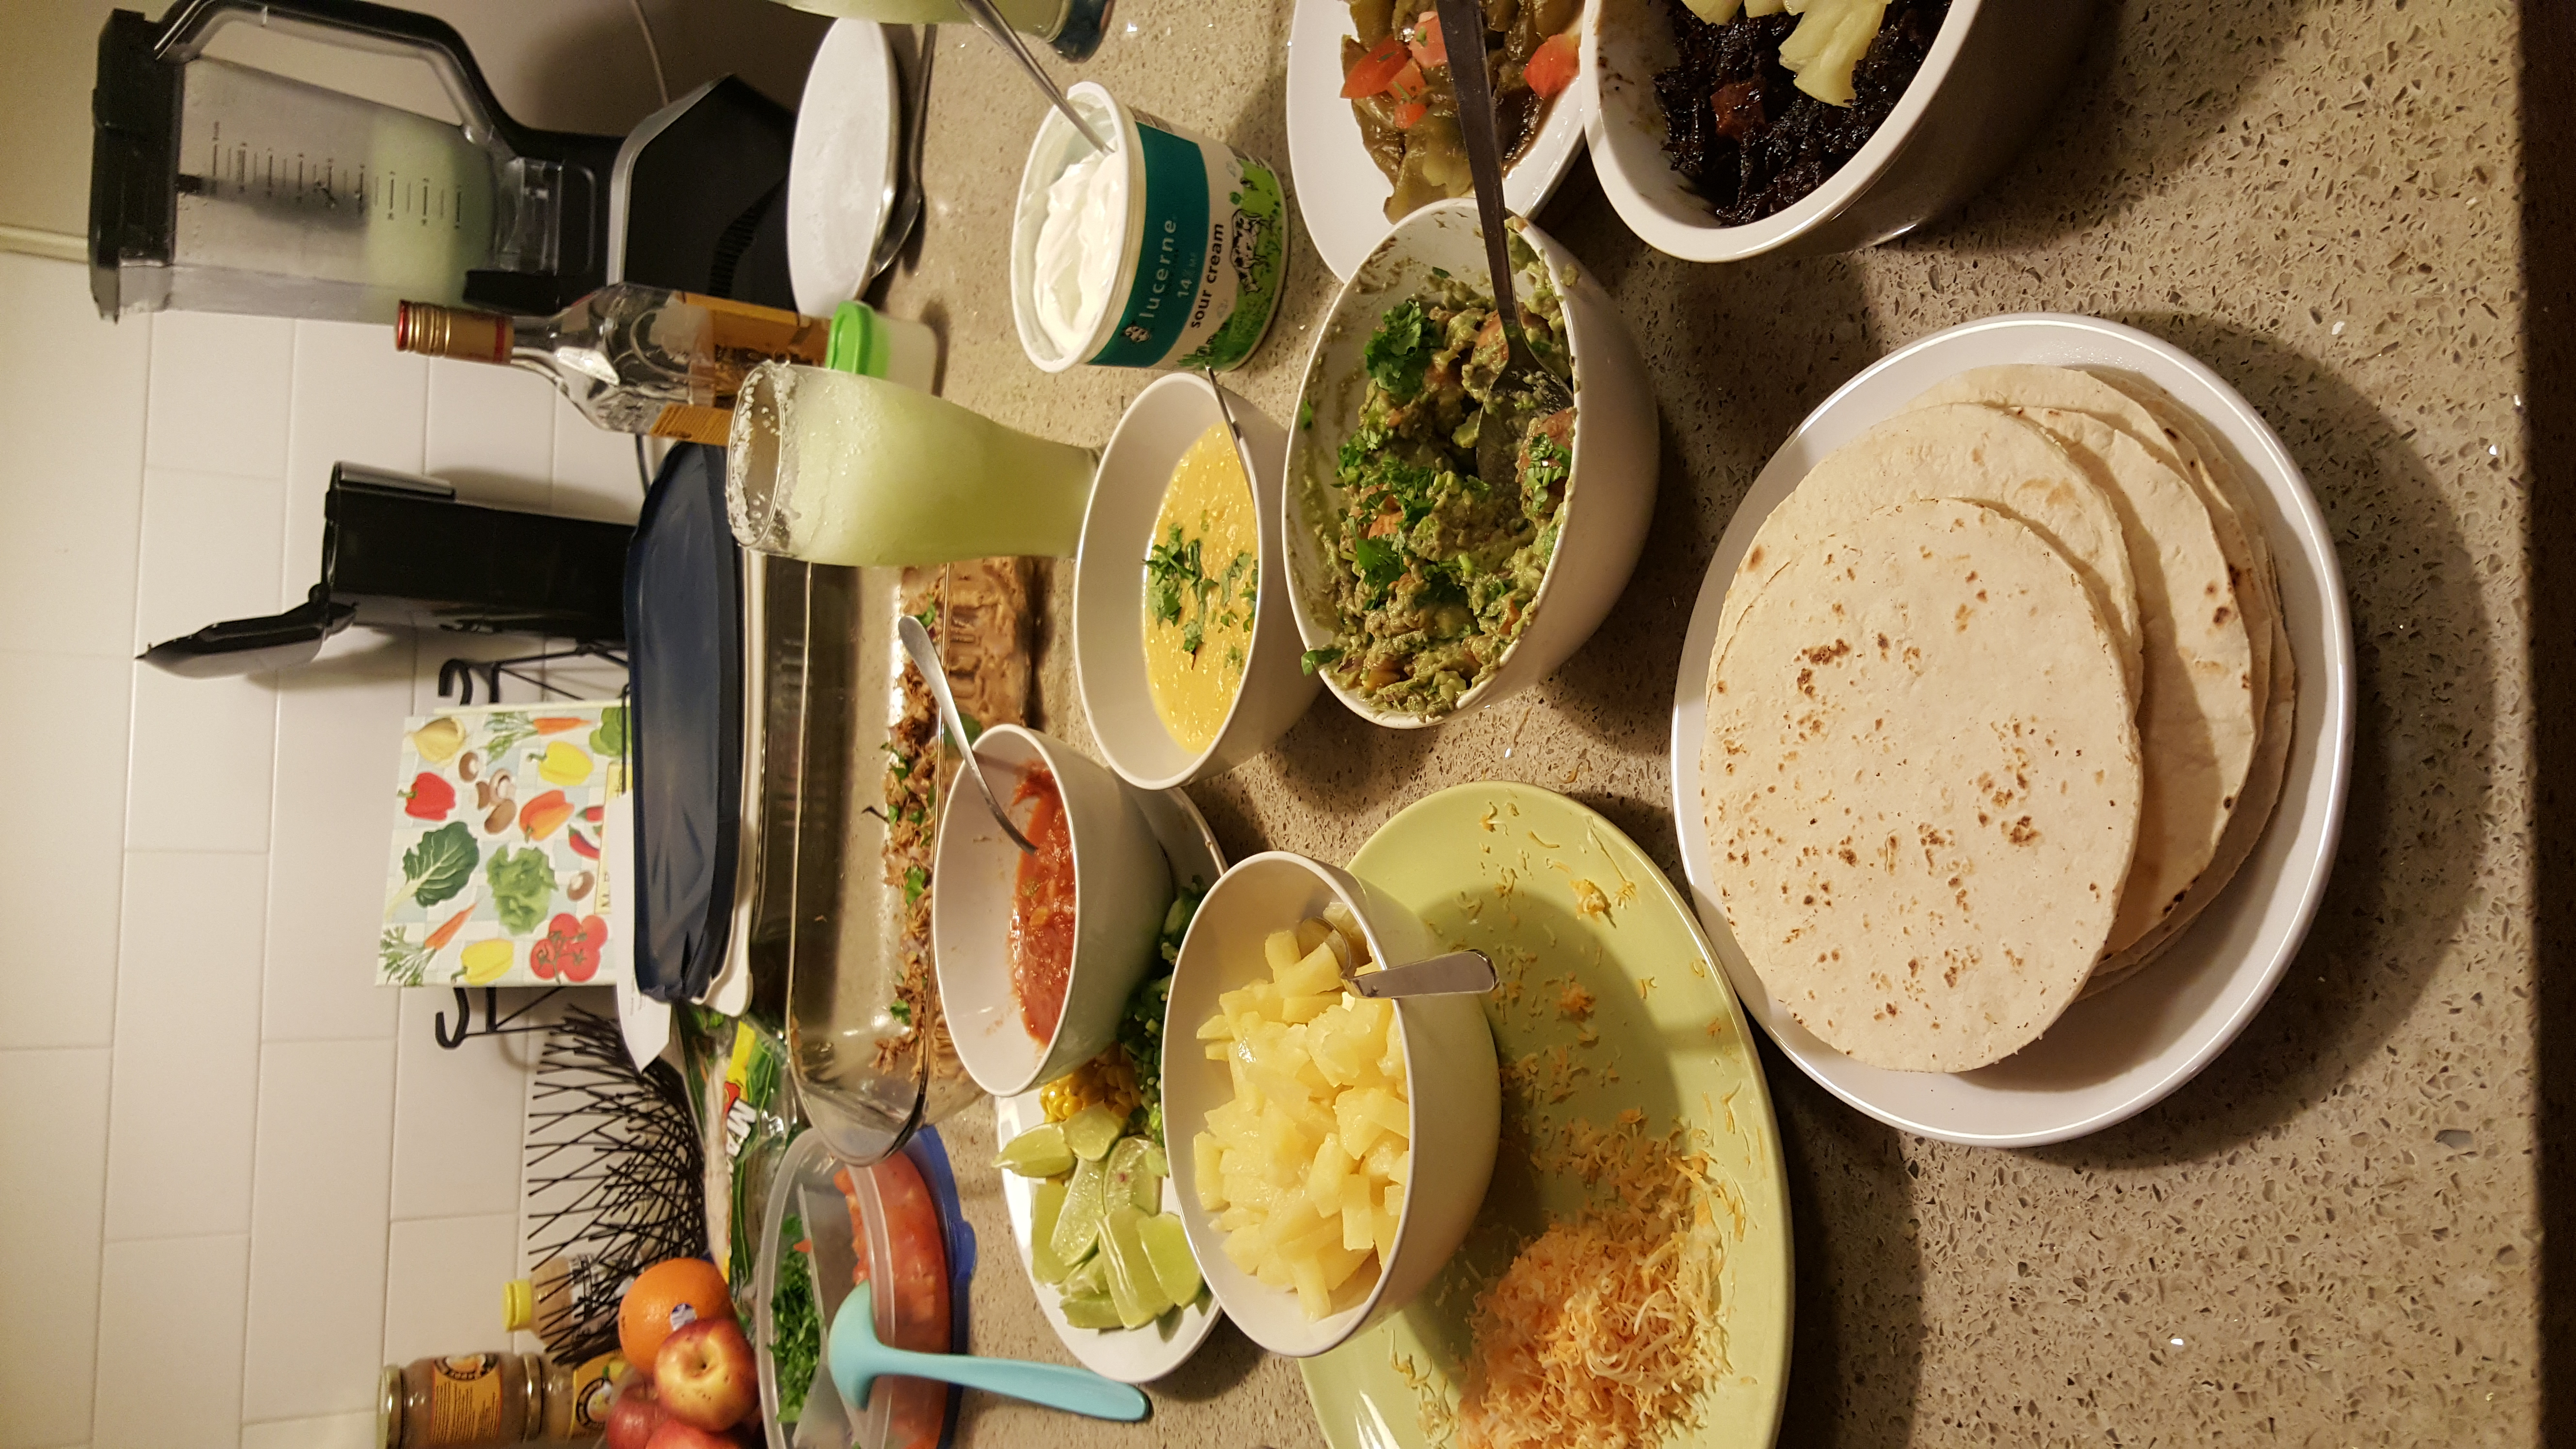
\includegraphics{/home/rachel/Documents/Cookbook/Pictures/20161126_202812.jpg}}
\newgeometry{left=0cm,bottom=0cm,top=0cm,right=0cm}
\newpage
\begin{figure}[]
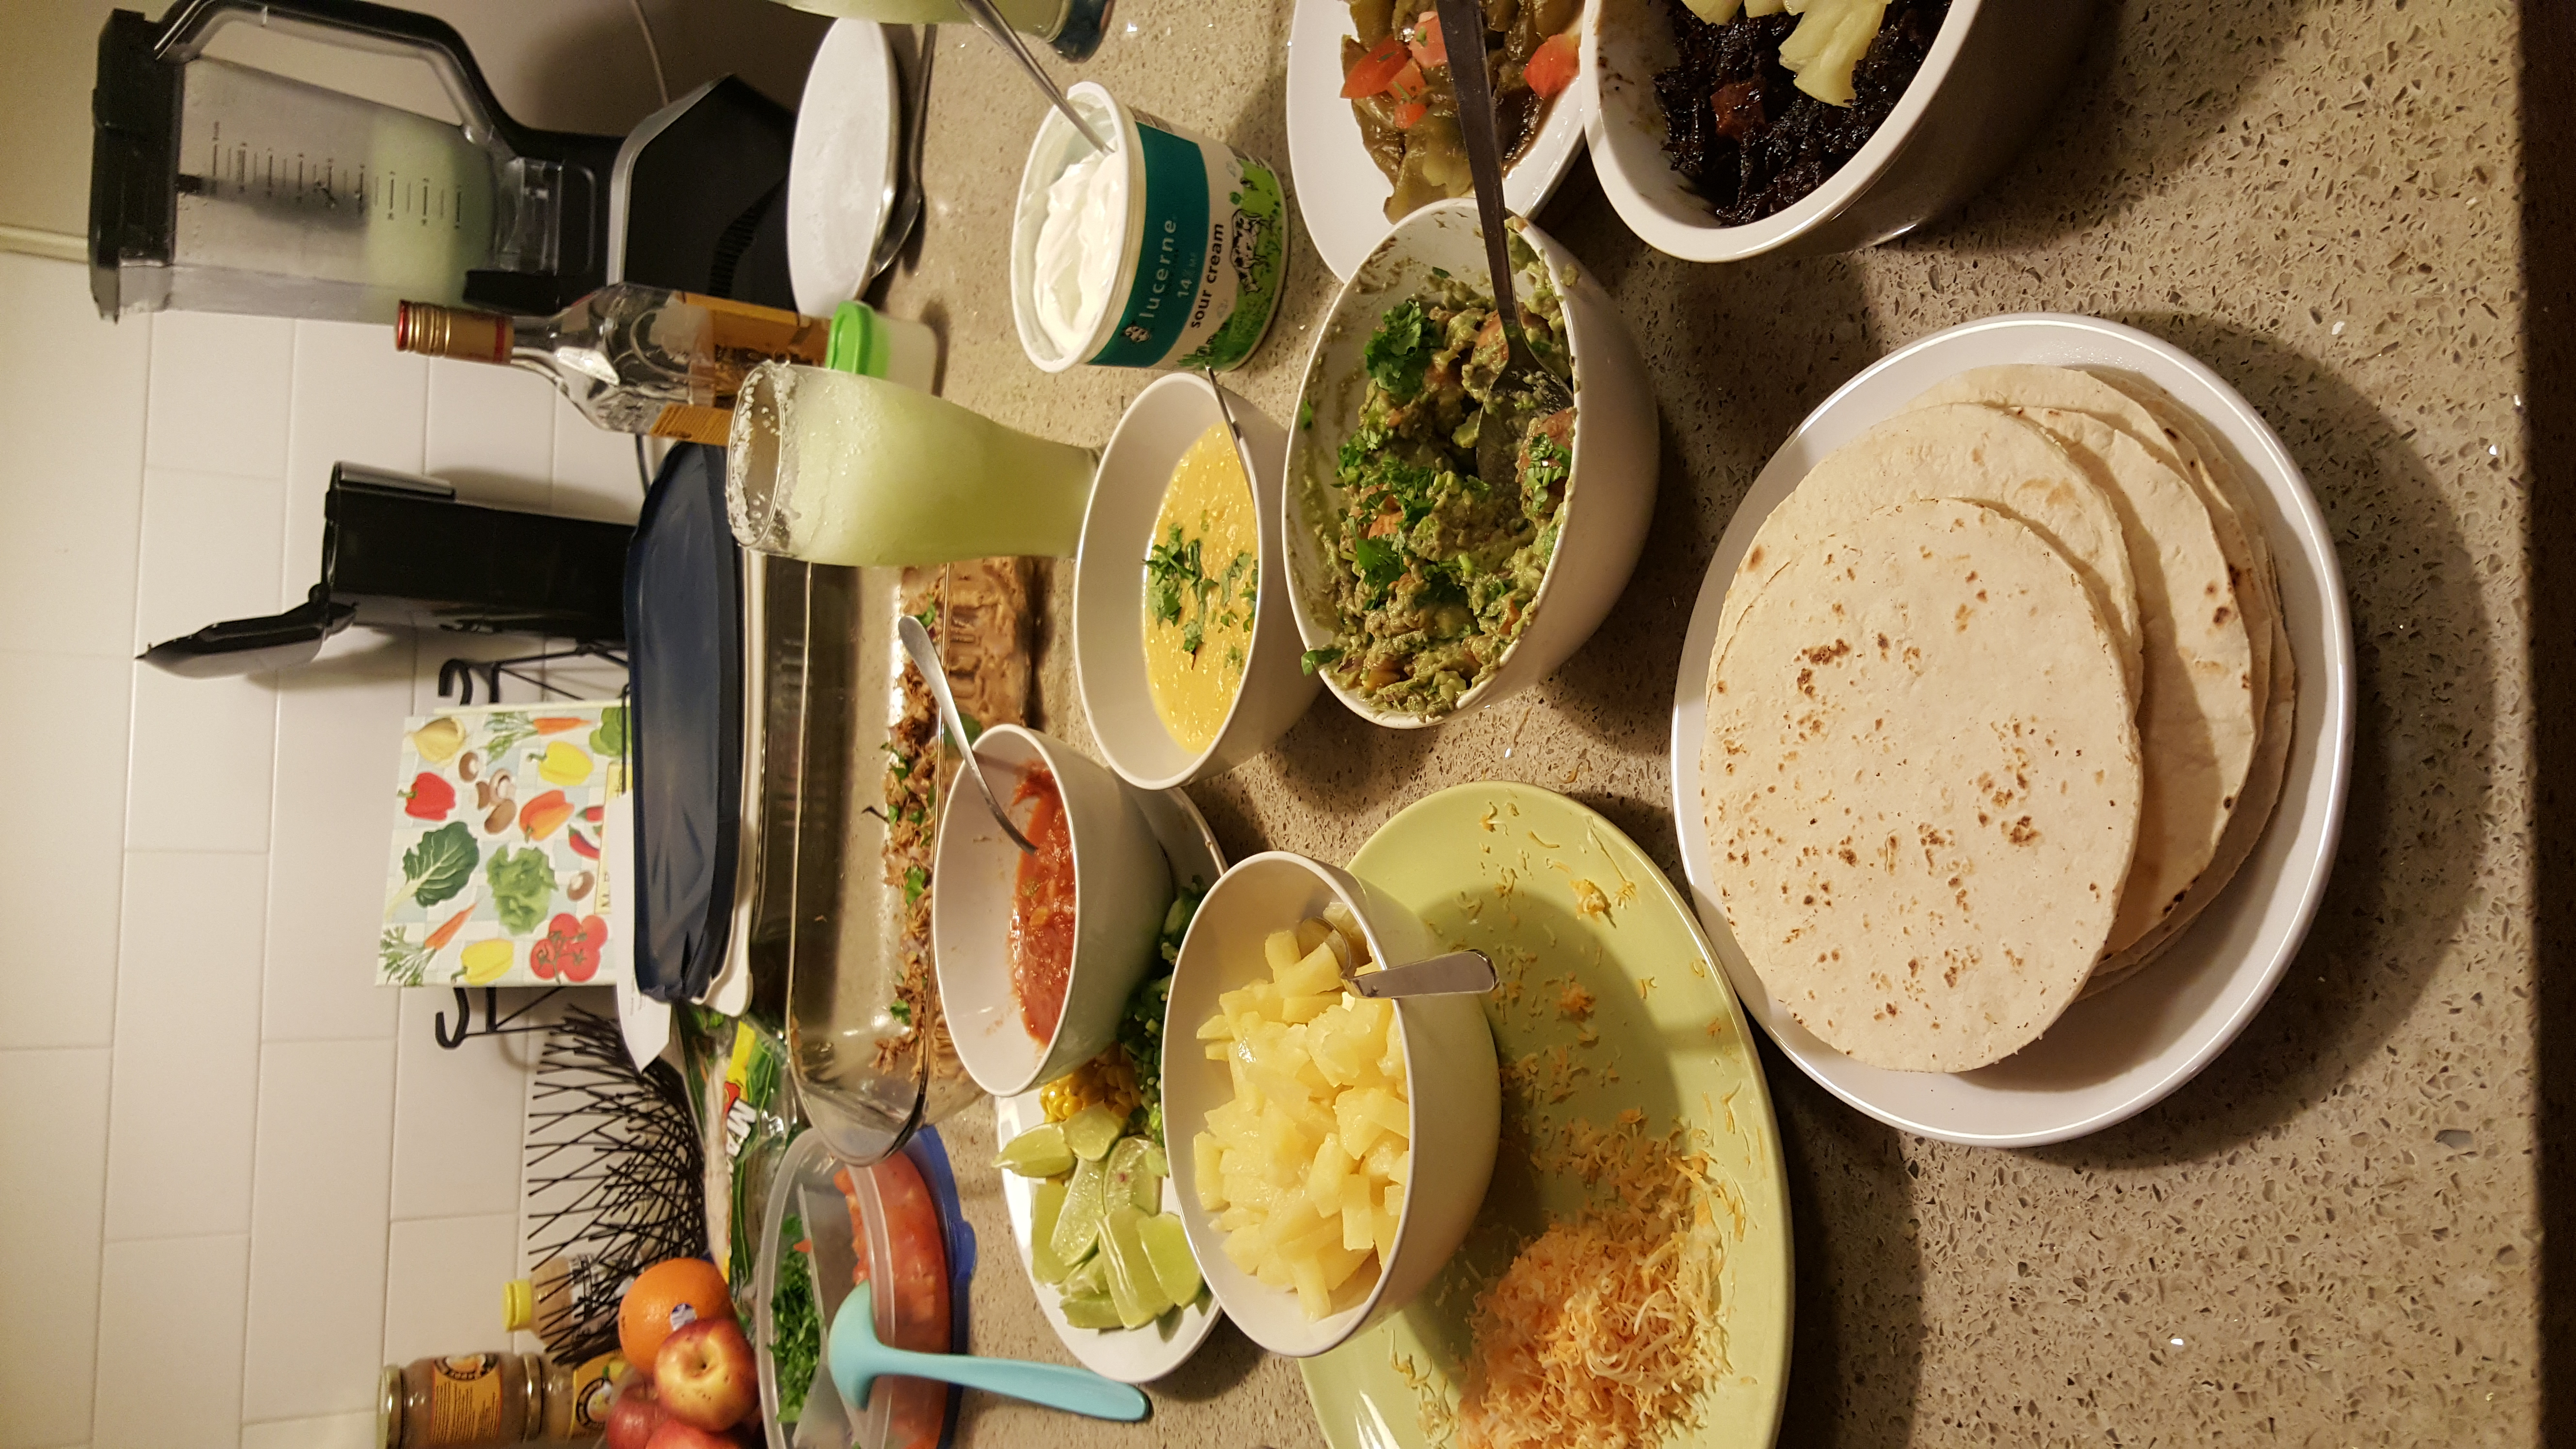
\includegraphics[trim = 1500 0 0 0, angle=-90, clip=true, width=\textwidth]{/home/rachel/Documents/Cookbook/Pictures/20161126_202812.jpg}
\end{figure}
\restoregeometry
\clearpage
\newpage
\newgeometry{right=0cm}




% recipe title
\section*{\fontsize{25}{15}\selectfont Taco Toppings}
\addcontentsline{toc}{section}{Taco Toppings}


% side figures
\begin{wrapfigure}{r}{0.5\textwidth}
\
  \begin{center}
 	\hfill\begin{minipage}{.5\textwidth}\centering
 	\vspace*{-5cm}
		\includegraphics[trim = 0 0 0 0, clip=true, width=0.8\textwidth]{/home/rachel/Documents/Cookbook/Pictures/20161126_204028.jpg}

		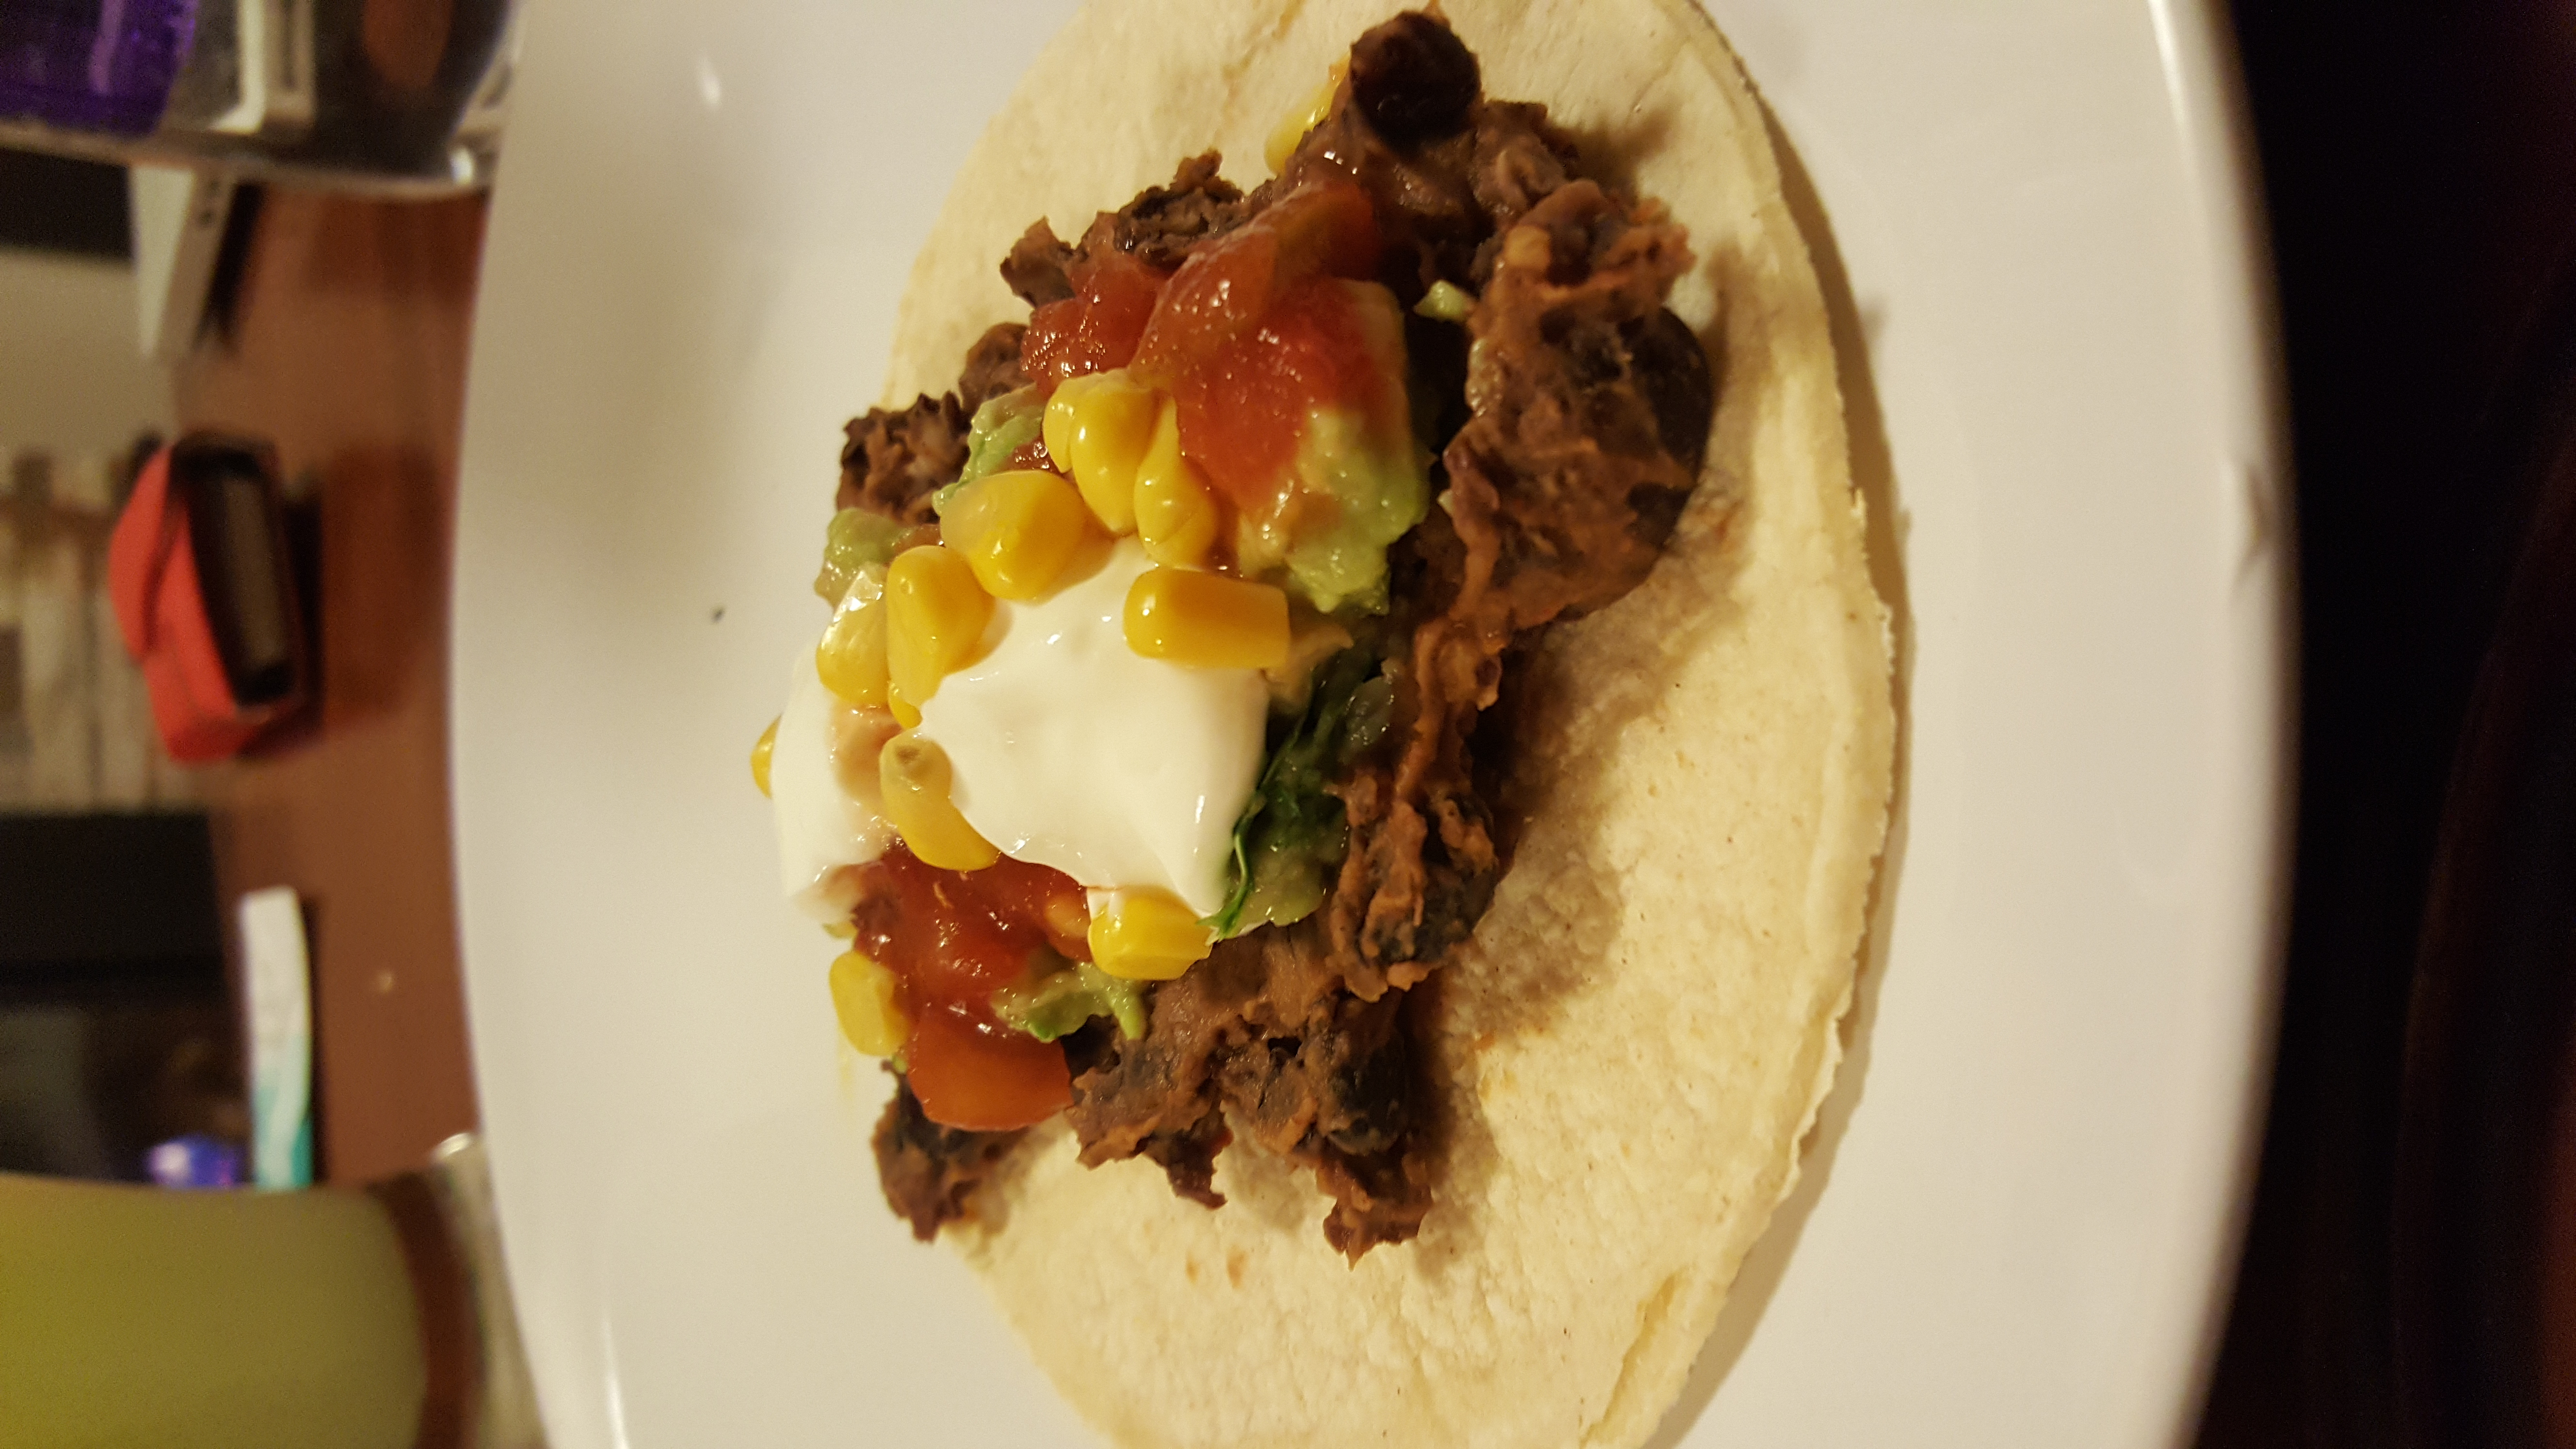
\includegraphics[trim = 500 0 0 0,   angle=-90, clip=true, width=0.8\textwidth]{/home/rachel/Documents/Cookbook/Pictures/20161126_203953.jpg}

		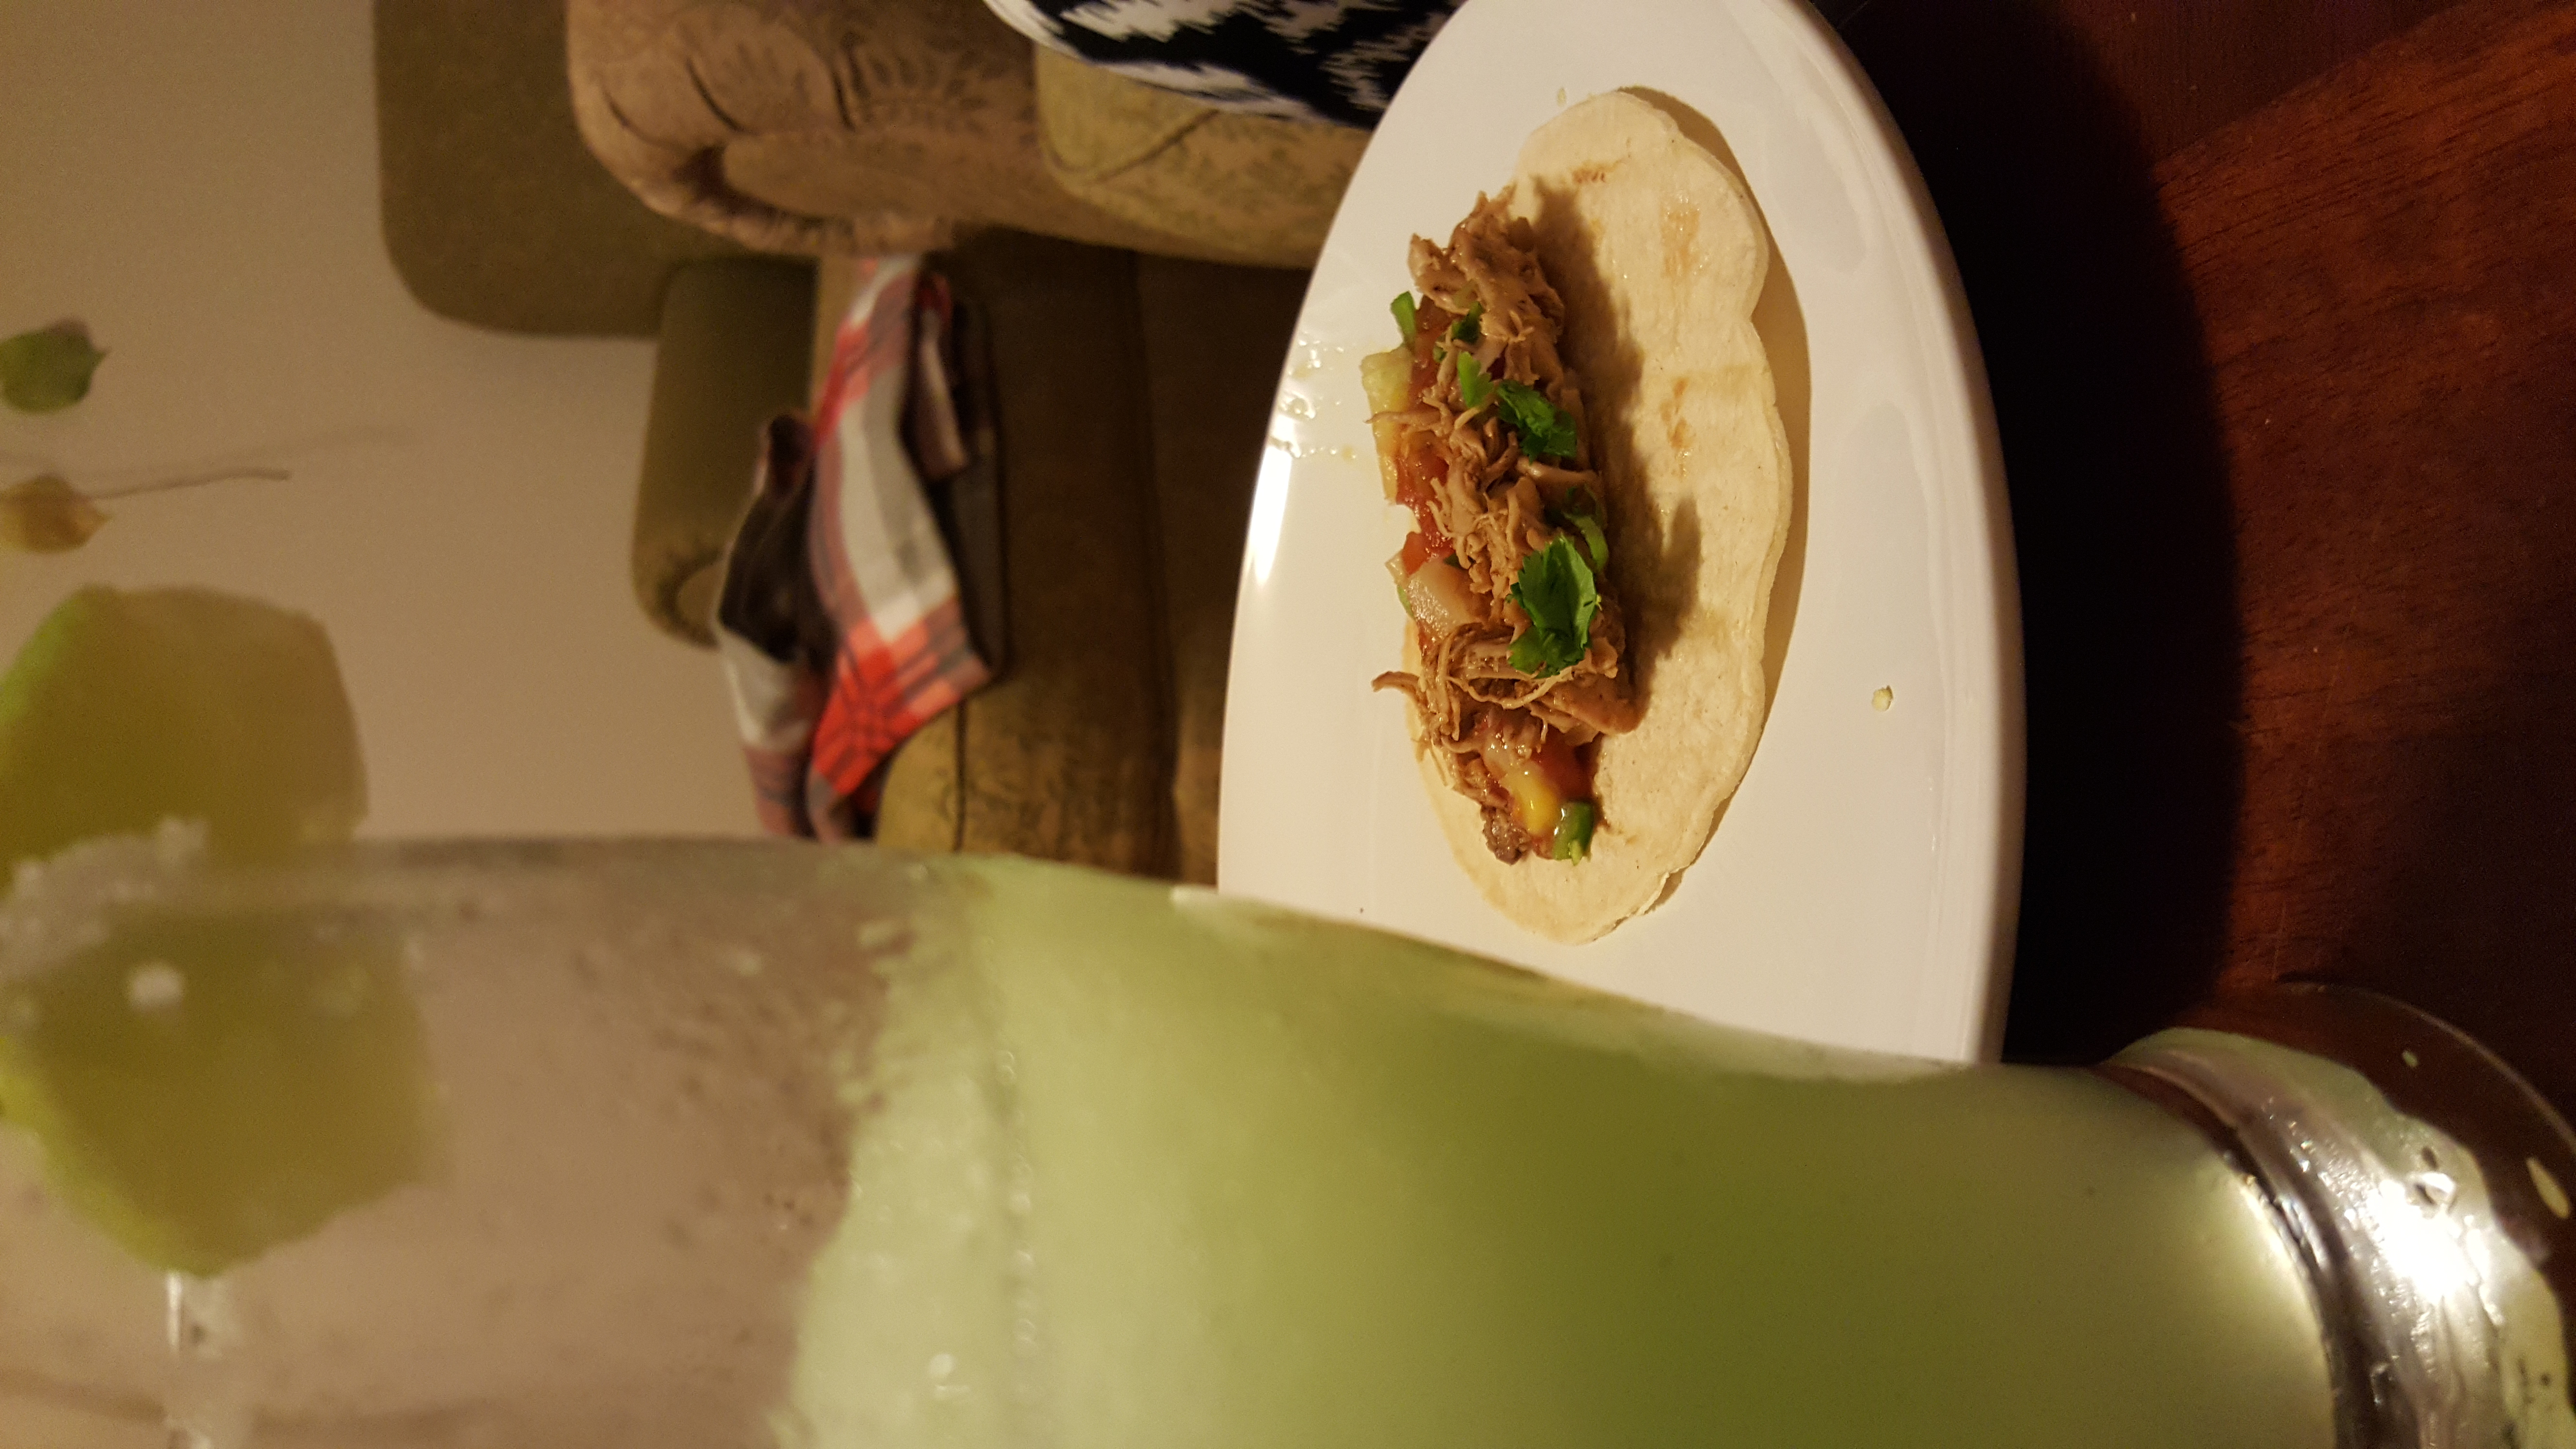
\includegraphics[trim = 1900 0 0 0, angle=-90, clip=true, width=0.8\textwidth]{/home/rachel/Documents/Cookbook/Pictures/20161126_204008.jpg}
	\end{minipage}  
	\end{center}

\end{wrapfigure}



% actual recipe
\vspace{5mm}

Here are all the things we included on taco night.
 
\vspace{5mm}
{\fontfamily{lmss}\selectfont 
    \begin{itemize}[noitemsep]
    
      \item[] Refried beans
      \item[] Pineapple
      \item[] Jalapenos
      \item[] Cheddar cheese
      \item[] Sour cream
      \item[] Salsa
      \item[] Cilantro
      \item[] Roasted pepper
      \item[] Corn
      \item[] Limes
      \item[] Green onion
      
    \end{itemize}
    }
\vspace{5mm}
   

\restoregeometry


\end{document}